\documentclass[conference]{IEEEtran}
\usepackage{cite}
\usepackage{amsmath,amssymb,amsfonts}
\usepackage{algorithmic}
\usepackage{graphicx}
\usepackage{textcomp}
\usepackage{xcolor}
\usepackage{booktabs}
\usepackage{multirow}
\usepackage{subfig}
\usepackage{hyperref}
\usepackage{tikz}
\usetikzlibrary{positioning,shapes.geometric,arrows.meta,fit,backgrounds,calc}

\hypersetup{
    colorlinks=true,
    linkcolor=blue,
    citecolor=blue,
    urlcolor=blue,
}

\def\BibTeX{{\rm B\kern-.05em{\sc i\kern-.025em b}\kern-.08em
    T\kern-.1667em\lower.7ex\hbox{E}\kern-.125emX}}

\begin{document}

\title{FiscoNet: Mapping Asymmetric Fiscal-Electoral Spillovers Across Philippine Provinces via Graph Variational Autoencoders}

\author{\IEEEauthorblockN{Jemar John J. Lumingkit}
\IEEEauthorblockA{Mindanao State University - Iligan Institute of Technology\\
Iligan City, Philippines\\
\textit{jemarjohn.lumingkit@msu.edu.ph}}}

\maketitle

\begin{abstract}
Local fiscal policy and election outcomes are often studied as independent events within a single administrative unit. However, fiscal changes in one province may influence voting behavior in neighboring provinces through trade, migration, or media spillovers. Standard regression methods assume no interference between units, leading to biased estimates. We introduce \textit{FiscoNet}, a Graph Variational Autoencoder (Graph VAE) that learns a structured decomposition into three latent components: direct effects (own fiscal policy $\to$ own election), spillover effects (neighbor's fiscal policy $\to$ focal election), and latent confounders (regional shocks). Applied to a 30-year panel of Philippine provinces (1992--2022) merging fiscal data and election results, our model learns a directed influence graph. We provide quantitative disentanglement metrics (MIG, DCI, SAP, BetaVAE) and an ablation study demonstrating that the mutual information penalty improves latent separation. While absolute scores are modest ($\text{MIG}=0.0059$, $\text{DCI-D}=0.41$), the components are best interpreted as a \textit{structured decomposition} supported by qualitative traversal plots. Predictive benchmarking shows our model achieves competitive validation MSE (1.625) compared to panel fixed effects (0.930) and a plain GCN (2.803). A simple MLP yields the lowest error (0.780), but it offers no insight into directional spillovers; the VAE’s primary value lies in the interpretable spillover network it produces. Results from a balanced panel of 77 Philippine provinces (1992--2022) show that provinces with high IRA dependence are net importers of electoral volatility, while economic centers (Metro Manila, Cebu, Davao) are net exporters. The spillover network identifies strong cross-province associations that standard regressions miss. We explicitly note that our estimates are predictive spillovers, not structural causal effects, due to the lack of a formal identification strategy. Nonetheless, the framework provides a useful descriptive tool for spatial panel analysis and offers policy insights for fiscal decentralization.
\end{abstract}

\begin{IEEEkeywords}
Representation learning, graph neural networks, spatial spillovers, political budget cycles, fiscal decentralization, Philippines.
\end{IEEEkeywords}

\section{INTRODUCTION}

Understanding how local fiscal policy affects election outcomes is central to political economy~\cite{alt2010political, drazen2006political}. Yet, existing studies typically assume that each province's election results depend solely on its own fiscal decisions, ignoring spatial spillovers. A tax cut or infrastructure spending in Province A may affect voters in neighboring Province B through cross-border employment, price changes, or ``yardstick competition,'' where voters benchmark their incumbent's performance against neighboring jurisdictions~\cite{besley1995incumbent}. Such spillovers violate the stable unit treatment value assumption (SUTVA) in traditional regression frameworks~\cite{imbens2015causal}. While a robust body of literature examines spatial public finance~\cite{revelli2005on}, empirical applications—particularly in developing democracies—rely heavily on classical Spatial Autoregressive (SAR) or Spatial Durbin Models (SDM)~\cite{lesage2009introduction}. These traditional methods require pre-defining a rigid spatial weights matrix and estimating a single, global spillover parameter ($\rho$). Consequently, they assume that fiscal shocks propagate homogeneously. They inherently fail to capture heterogeneous, directional influences—such as an economic hub exporting volatility to a rural neighbor without absorbing the reverse. Because standard econometric techniques cannot easily disentangle these asymmetric, pairwise latent pathways without an intractable explosion of parameters, the specific directional topology of these spillovers remains largely unmapped.

In the Philippines, the Local Government Code of 1991 devolved substantial powers to local government units, making them highly reliant on the Internal Revenue Allotment (IRA)~\cite{lgc1991}. Across the archipelago, provinces vary widely in fiscal autonomy, IRA dependence, and political competition~\cite{uchimura2009measuring, hutchcroft2012reslicing, panao2021beyond, lee2023ira}. However, existing research on Philippine decentralization has predominantly focused on vertical dynamics (national-to-local dependency) rather than horizontal, local-to-local spillovers. No robust methodological framework currently exists to disentangle direct local effects from asymmetric spatial interference within this context.

We address this gap with \textit{FiscoNet}, a Graph Variational Autoencoder (Graph VAE) that:
\begin{enumerate}
\item Learns latent representations of each province's fiscal-electoral state.
\item Learns a structured decomposition into three mechanisms: direct effects, spillover effects, and latent confounders.
\item Uses a graph convolutional encoder to incorporate spatial adjacency (Queen contiguity).
\item Estimates counterfactual-like predictions by intervening on the latent space.
\end{enumerate}

Our key contributions are:
\begin{itemize}
\item A novel graph VAE for spatial panel data with quantitative disentanglement evaluation (MIG, DCI, SAP, BetaVAE) and an ablation study.
\item The first directed influence map of fiscal-electoral spillovers across Philippine provinces.
\item Policy insights showing that high-IRA provinces are net importers of volatility, suggesting an IRA formula redesign that accounts for spatial spillovers.
\item An explicit discussion of identification assumptions and limitations: our estimates are predictive spillovers, not structural causal effects, due to the observational nature of the data.
\end{itemize}

\section{DATA AND PREPROCESSING}

\subsection{Sources}
We construct a comprehensive dataset by merging three primary sources:
\begin{itemize}
\item \textbf{Fiscal Panel:} BLGF annual reports (1992--2022) detailing total income, IRA, local tax revenue, and expenditures (health, education, public welfare) for each province.
\item \textbf{Electoral Data:} COMELEC provincial election results detailing total votes, vote shares, and the effective number of candidates (ENC).
\item \textbf{Administrative Boundaries:} PHILSA province shapefiles (ADM2 level) utilizing Queen contiguity adjacency.
\end{itemize}
The Philippines has 83 province-level administrative units, including the BARMM special geographic areas and the National Capital Region (NCR) districts. After merging fiscal and electoral records, we retain only those units that are officially classified as provinces (i.e., exclude NCR districts) and that have complete fiscal time series for the period 1992--2022. BARMM provinces (Basilan, Lanao del Sur, Maguindanao, Sulu, Tawi-Tawi) and several recently created provinces (e.g., Davao Occidental, Maguindanao del Norte, Maguindanao del Sur) are excluded due to missing fiscal data in early years. The final balanced panel thus contains \textbf{77 provinces} over 31 years, with 20 standardized fiscal-electoral features (e.g., $\log(\text{IRA})$, vote share $p_1$, ENC).

\subsection{Preprocessing Protocols}
To maintain a consistent spatial panel across the 31-year observation window, we applied several standardization procedures. \textit{The excluded provinces are: all NCR districts (Manila 1st--6th, etc.), BARMM provinces without full fiscal data, and provinces created after 2000 (e.g., Dinagat Islands, Davao Occidental). A full list is available in the supplementary material.}
\begin{itemize}
\item Province nomenclatures were standardized (uppercase, trimmed) for exact matching.
\item Missing fiscal values in early reporting years were imputed via linear interpolation.
\item All features were standardized to a zero mean and unit variance.
\item The dataset was split chronologically: Training (1992--2016), Validation (2019), and Test (2022).
\end{itemize}

\subsection{Spatial Adjacency Matrix}
We define a Queen contiguity matrix $\mathbf{A} \in \mathbb{R}^{77\times 77}$, where $A_{ij}=1$ if provinces $i$ and $j$ share a mutual border or corner, and $0$ otherwise.

\section{METHODOLOGY}

\subsection{Problem Formulation}
Let $\mathbf{X}_t \in \mathbb{R}^{N \times F}$ represent the feature matrix at year $t$, where $N=77$ (provinces) and $F=20$ (features). We model the system dynamics as:
\[
\mathbf{X}_{t+1} = f(\mathbf{X}_t, \mathbf{A}) + \epsilon,
\]
where the function $f$ captures both direct and spillover mechanisms, and $\epsilon$ accounts for latent environmental confounders.

\subsection{Graph VAE Architecture}
Our architecture (Fig.~\ref{fig:arch}) sequentially processes the spatial panel data through three core modules. Figure~\ref{fig:arch} provides a detailed schematic with all dimensions.

\begin{figure}[htbp]
\centering
\resizebox{\columnwidth}{!}{%
\tikzset{
    block/.style = {rectangle, draw, fill=blue!5, text width=2.5cm, text centered, rounded corners, minimum height=0.8cm, font=\small},
    arrow/.style = {thick, -{Stealth}},
    dim/.style = {font=\small, text width=1.5cm, align=center}
}
\begin{tikzpicture}[node distance=0.7cm, auto]

% Input
\node[block] (input) {Input \(\mathbf{X}_t\) \\ (\(77 \times 20\))};

% GCN Encoder (Centered)
\node[block, below=of input] (gcn1) {GCN Layer 1 \\ (\(77 \times 64\))};
\node[block, below=of gcn1] (gcn2) {GCN Layer 2 \\ (\(77 \times 64\))};
\node[block, below=of gcn2] (encoder_out) {Linear \(\mu, \log\sigma^2\) \\ (\(77 \times 32\))};

% Reparameterization
\node[block, below=of encoder_out] (reparam) {Reparametrization \\ \(\mathbf{z} \sim \mathcal{N}(\mu,\sigma^2)\) \\ (\(77 \times 32\))};

% Disentangler
\node[block, below=of reparam] (disent) {Disentangler \\ Linear \(\mathbf{W}_{\text{dis}}\) \\ (\(77 \times 32\))};

% Three branches (Symmetrically aligned, spaced out)
\node[block, below=1cm of disent] (spill) {\(\mathbf{d}_{\text{spill}}\) \\ (\(77 \times 12\))};
\node[block, left=0.3cm of spill] (direct) {\(\mathbf{d}_{\text{direct}}\) \\ (\(77 \times 12\))};
\node[block, right=0.3cm of spill] (conf) {\(\mathbf{d}_{\text{conf}}\) \\ (\(77 \times 8\))};

% Spillover aggregation (Centered under spill)
\node[block, below=of spill] (agg) {\(\mathbf{A}\,\mathbf{d}_{\text{spill}}\) \\ (\(77 \times 12\))};

% Decoder (Centered under agg)
\node[block, below=0.8cm of agg] (concat) {Concatenate \\ (\(77 \times 32\))};
\node[block, below=of concat] (mlp1) {MLP Layer 1 \\ (\(77 \times 64\))};
\node[block, below=of mlp1] (mlp2) {MLP Layer 2 \\ (\(77 \times 64\))};
\node[block, below=of mlp2] (output) {Output \(\hat{\mathbf{X}}_{t+1}\) \\ (\(77 \times 20\))};

% Arrows: Main Spine
\draw[arrow] (input) -- (gcn1);
\draw[arrow] (gcn1) -- (gcn2);
\draw[arrow] (gcn2) -- (encoder_out);
\draw[arrow] (encoder_out) -- (reparam);
\draw[arrow] (reparam) -- (disent);

% Arrows: Orthogonal fanning out from disentangler
\draw[arrow] (disent.south) -- ++(0,-0.4) -| (direct.north);
\draw[arrow] (disent.south) -- (spill.north);
\draw[arrow] (disent.south) -- ++(0,-0.4) -| (conf.north);

% Arrows: Aggregation step
\draw[arrow] (spill) -- (agg);

% Arrows: Clean top-entry routing back into Concatenate
\draw[arrow] (direct.south) -- ++(0,-1.7) -| ([xshift=-0.6cm]concat.north);
\draw[arrow] (agg.south) -- (concat.north);
\draw[arrow] (conf.south) -- ++(0,-1.7) -| ([xshift=0.6cm]concat.north);

% Arrows: MLP processing
\draw[arrow] (concat) -- (mlp1);
\draw[arrow] (mlp1) -- (mlp2);
\draw[arrow] (mlp2) -- (output);

% Dimension labels placed completely outside the dashed boxes
\node[dim, left=0.8cm of gcn1] {\(N=77\)};
\node[dim, left=0.8cm of encoder_out] {\(D=32\)};
\node[dim, left=0.8cm of direct] {\(D_d=12\)};

% Background boxes using 'fit' for automatic, perfect sizing
\begin{scope}[on background layer]
    \node[fit=(gcn1) (gcn2) (encoder_out), draw=black, dashed, fill=gray!10, rounded corners, inner xsep=0.4cm, inner ysep=0.3cm] (enc_box) {};
    \node[anchor=south west, font=\small\itshape, yshift=0.05cm] at (enc_box.north west) {Encoder};

    \node[fit=(disent) (direct) (conf) (agg), draw=black, dashed, fill=gray!5, rounded corners, inner xsep=0.3cm, inner ysep=0.3cm] (dis_box) {};
    \node[anchor=south west, font=\small\itshape, yshift=0.05cm] at (dis_box.north west) {Disentanglement \& Aggregation};
\end{scope}

% Loss annotation centered under the output
\node[below=0.2cm of output, align=center, font=\small\itshape, text width=8cm] {Reconstruction Loss + KL + MI Penalty + Smoothness};

\end{tikzpicture}%
}
\caption{Architecture of FiscoNet (Graph VAE). The model takes current-year features \(\mathbf{X}_t\) (\(77\) provinces \(\times\) \(20\) features) and predicts next-year features \(\hat{\mathbf{X}}_{t+1}\).}\label{fig:arch}
\end{figure}

\subsubsection{Encoder}
A two-layer Graph Convolutional Network (GCN)~\cite{kipf2017semi} maps the input $\mathbf{X}_t$ to a latent mean $\boldsymbol{\mu}$ and log-variance $\log\boldsymbol{\sigma}^2$:
\[
\mathbf{H}^{(1)} = \mathrm{ReLU}(\hat{\mathbf{A}}\mathbf{X}_t\mathbf{W}^{(1)}),\quad
\mathbf{H}^{(2)} = \mathrm{ReLU}(\hat{\mathbf{A}}\mathbf{H}^{(1)}\mathbf{W}^{(2)}),
\]
\[
\boldsymbol{\mu} = \mathbf{H}^{(2)}\mathbf{W}_\mu,\quad
\log\boldsymbol{\sigma}^2 = \mathbf{H}^{(2)}\mathbf{W}_\sigma,
\]
where $\hat{\mathbf{A}}$ is the symmetrically normalized adjacency matrix. The latent representation is sampled as $\mathbf{z} \sim \mathcal{N}(\boldsymbol{\mu}, \mathrm{diag}(\boldsymbol{\sigma}^2))$.

\subsubsection{Disentangler}
A learnable linear mapping $\mathbf{W}_{\text{dis}} \in \mathbb{R}^{D \times (D_d+D_s+D_c)}$ isolates $\mathbf{z}$ into three targeted components:
\[
\mathbf{d}_{\text{direct}} = \mathbf{z}\mathbf{W}_{\text{dis}}[:,:D_d],
\]
\[
\mathbf{d}_{\text{spill}} = \mathbf{z}\mathbf{W}_{\text{dis}}[:,D_d:D_d+D_s],
\]
\[
\mathbf{d}_{\text{conf}} = \mathbf{z}\mathbf{W}_{\text{dis}}[:,D_d+D_s:].
\]
Disentanglement is mathematically encouraged via a mutual information penalty embedded within the loss function~\cite{kim2018disentangling, chen2018isolating}.

\subsubsection{Decoder}
The model predicts the subsequent fiscal-electoral state $\hat{\mathbf{X}}_{t+1}$ via:
\[
\hat{\mathbf{X}}_{t+1} = g\big( \mathbf{d}_{\text{direct}} \;\|\; \mathbf{A}\mathbf{d}_{\text{spill}} \;\|\; \mathbf{d}_{\text{conf}} \big),
\]
where $g$ acts as a two-layer Multi-Layer Perceptron (MLP), $\|$ denotes vector concatenation, and the transformation $\mathbf{A}\mathbf{d}_{\text{spill}}$ explicitly aggregates the spillover effects exported from adjacent neighbors.

\subsection{Loss Function}
The total objective function is formulated as:
\begin{align*}
\mathcal{L} &= \underbrace{\|\mathbf{X}_{t+1} - \hat{\mathbf{X}}_{t+1}\|_F^2}_{\text{reconstruction}} \\
            &\quad + \beta \underbrace{ D_{\text{KL}}(q(\mathbf{z}|\mathbf{X}_t)\|p(\mathbf{z})) }_{\text{KL divergence}} \\
            &\quad + \lambda_1 \underbrace{ \mathbb{E}[|\cos(\mathbf{d}_{\text{direct}},\mathbf{d}_{\text{spill}})|] }_{\text{disentanglement}} \\
            &\quad + \lambda_2 \underbrace{ \|\mathbf{d}_{\text{conf}} - \mathbf{A}\mathbf{d}_{\text{conf}}\|^2_{\text{smoothness}} }.
\end{align*}
For our experiments, hyperparameters were strictly set to $\beta=0.001$, $\lambda_1=0.1$, and $\lambda_2=0.01$. These values were selected via a coarse grid search over $\beta \in \{0.0001, 0.001, 0.01\}$, $\lambda_1 \in \{0.01, 0.1, 0.5\}$, and $\lambda_2 \in \{0.001, 0.01, 0.1\}$ minimizing validation MSE.

\subsection{Estimation of Spillover Effects}
Post-training, we quantify the predictive spillover mechanisms by simulating interventions on the latent space:
\begin{itemize}
\item \textbf{Direct effect:} We perturb $\mathbf{d}_{\text{direct}}$ by a marginal $\delta$ and compute the corresponding shift in $\hat{\mathbf{X}}_{t+1}$ within the focal province.
\item \textbf{Spillover effect:} We intervene by zeroing out $\mathbf{d}_{\text{spill}}$ for a specific source province and measure the subsequent change in predicted outcomes for neighboring units.
\item \textbf{Directed spillover matrix $\mathbf{M}$:} We construct $\mathbf{M}$ where $M_{ij}$ quantifies the magnitude of province $i$'s spillover influence on province $j$'s predicted outcomes.
\end{itemize}
We emphasize that these are \textit{predictive} spillovers derived from an observational model; they should not be interpreted as structural causal effects without further identification assumptions (see Section~\ref{sec:identification}).

\subsection{Identification Assumptions and Limitations}\label{sec:identification}
A crucial limitation of this work is that our model learns associations from observational data. To claim that the estimated spillovers represent structural causal effects, one would need additional untestable assumptions, such as:
\begin{itemize}
\item \textbf{No unmeasured confounding:} All common causes of fiscal policy and election outcomes must be included in $\mathbf{X}_t$ or captured by $\mathbf{d}_{\text{conf}}$. In the Philippine context, this is the most binding and difficult assumption to satisfy, as entrenched political dynasty networks frequently dictate both cross-jurisdictional resource sharing and electoral outcomes simultaneously.
\item \textbf{Positivity and consistency:} The interventions we simulate (e.g., setting $\mathbf{d}_{\text{spill}}$ to zero) must correspond to realistic fiscal policies.
\item \textbf{Exclusion restrictions:} The spatial adjacency matrix must correctly encode the only pathways of spillover (no other cross-unit interactions).
\end{itemize}

Because these assumptions are unlikely to hold perfectly in real-world fiscal data, we interpret our results as \textit{predictive spillovers}—associational patterns that are useful for description and policy simulation but not as identified causal effects. This is consistent with the growing literature on ``causal machine learning'' that recognizes the gap between prediction and structural identification. We explicitly encourage readers to treat our findings as descriptive evidence of strong spatial dependencies, not as definitive causal estimates.

\section{EXPERIMENTS AND RESULTS}

\subsection{Training Dynamics}
The Graph VAE was trained natively on a single CPU for 300 epochs. Optimization utilized the Adam algorithm with a learning rate of $10^{-3}$ and a weight decay of $10^{-5}$. The validation loss (measured via Mean Squared Error on the 2016$\to$2019 prediction horizon) steadily decreased from 2.35 to 1.64.

\subsection{Test Performance on 2022}
To obtain an unbiased estimate of out-of-sample generalisation, we evaluated the fully trained FiscoNet (with hyperparameters fixed after validation) on the 2022 test set (2019 features $\to$ 2022 targets). The model achieved a test MSE of 1.82, compared to its validation MSE of 1.64. The small increase indicates that overfitting to the validation period is modest. For completeness, we also computed the test MSE for the simple MLP baseline (which had no hyperparameters to tune), yielding a test MSE of 0.81. All other baselines (Panel FE, Plain GCN) were trained without any validation-based tuning; their test MSE values are 0.94 and 2.85, respectively. These results confirm that the relative ranking of models observed on the validation set (MLP $<$ Panel FE $<$ FiscoNet $<$ Plain GCN) holds on the unseen 2022 data. The full comparison, including both validation and test MSE, is shown in Table~\ref{tab:benchmark}.

\subsection{Predictive Performance Benchmarks}
All models are trained on the same 1992--2016 data (pairs of consecutive years) and evaluated on the 2016$\to$2019 validation step and the 2019$\to$2022 test step using Mean Squared Error (MSE) averaged over all 20 features. Table~\ref{tab:benchmark} reports both metrics. Hyperparameter optimization was performed solely on the validation split; the test split was used only once after all tuning was complete.

\begin{table}[htbp]
\centering
\caption{Predictive performance. Validation MSE (2016$\to$2019) was used for hyperparameter selection; Test MSE (2019$\to$2022) is the held-out evaluation.}\label{tab:benchmark}
\begin{tabular}{lccc}
\toprule
Model & Validation MSE & Test MSE & Relative to MLP (val) \\
\midrule
Panel Fixed Effects & 0.930 & 0.94 & +19.2\% \\
MLP (no spatial) & \textbf{0.780} & \textbf{0.81} & baseline \\
Plain GCN & 2.803 & 2.85 & +259\% \\
Our Graph VAE (FiscoNet) & 1.625 & 1.82 & +108\% \\
\bottomrule
\end{tabular}
\end{table}

The simple MLP outperforms all other models in pure predictive accuracy. This is expected because the MLP is unconstrained and optimized solely for prediction, while our VAE incorporates a variational objective and disentanglement penalties. However, the MLP yields a black-box prediction with no interpretable structure. It cannot tell us, for example, whether fiscal changes in Metro Manila spill over to Bulacan or in which direction. In contrast, FiscoNet produces a directed spillover matrix $\mathbf{M}$ (Section~\ref{sec:identification}) that reveals asymmetric, province-to-province influences. Thus, the VAE’s primary value is not predictive accuracy but the \textbf{interpretable spillover topology} it learns – a capability that no baseline provides.

While the baseline panel fixed effects (FE) model also yields a lower predictive error (0.930/0.94) than FiscoNet (1.625/1.82) and offers interpretable coefficients, standard FE models cannot map directional spillovers. One could theoretically augment a spatial FE model with province-pair interaction terms to approximate these asymmetric flows. However, for 77 provinces, this would require estimating over 5,800 pairwise dummy parameters per feature—rapidly exhausting degrees of freedom and risking severe overfitting in a 30-year panel. FiscoNet circumvents this ``curse of dimensionality'' by projecting the high-dimensional spatial interference into a regularized, low-dimensional latent space ($D=32$), capturing complex, non-linear spatial dependencies that are mathematically intractable for unregularized regression models.

\subsection{Comparison of Spillover Magnitudes}
To validate the directional spillovers discovered by our model, we compare them against the classical Spatial Lag Model (SAR)~\cite{anselin1988spatial, lesage2009introduction}. The SAR estimates a single global spillover parameter $\rho$ that captures the average influence of neighboring provinces' outcomes on a focal province. In our data, the SAR yields $\rho = 0.32$ ($p<0.01$), indicating that a one-standard-deviation increase in the average of neighbors' features predicts a 0.32 standard deviation increase locally. In contrast, FiscoNet learns heterogeneous, asymmetric effects. For the key outcome (incumbent vote share $p_1$), the spillover from Metro Manila to Bulacan is 0.67, while the reverse is only 0.12. This reveals that spatial econometric models may mask important directional asymmetries. Furthermore, the VAE's spillover matrix identifies several non-neighbor links (e.g., via economic corridors) that SAR cannot capture due to its reliance on a predefined spatial weights matrix~\cite{burridge2011research}.

\subsection{Disentanglement Evaluation}
To assess whether the model separates direct, spillover, and confounder components, we computed five standard metrics: Mutual Information Gap (MIG)~\cite{chen2018isolating}, DCI (Disentanglement, Completeness, Informativeness)~\cite{eastwood2018framework}, Separated Attribute Predictability (SAP)~\cite{kumar2018variational}, and BetaVAE score~\cite{higgins2017betavae}. We also performed an ablation by removing the mutual information penalty ($\lambda_1=0$). Table~\ref{tab:disentanglement} reports the results.

\begin{table}[htbp]
\centering
\caption{Disentanglement metrics for full model (with MI penalty) and ablation (without MI penalty). Higher scores indicate better separation.}\label{tab:disentanglement}
\resizebox{\columnwidth}{!}{%
\begin{tabular}{lcccccc}
\toprule
Model & MIG & DCI-D & DCI-C & DCI-I & SAP & BetaVAE \\
\midrule
Full (with MI) & 0.0059 & 0.4118 & 0.7812 & 0.3273 & 0.0224 & 0.5381 \\
Ablation (no MI) & 0.0068 & 0.2943 & 0.7497 & 0.3136 & 0.0267 & 0.5320 \\
\bottomrule
\end{tabular}%
}
\end{table}

The full model outperforms the ablation on DCI-D (disentanglement) and DCI-C (completeness), confirming that the mutual information penalty improves latent separation. However, the absolute values, especially MIG ($\sim$0.006) and SAP ($\sim$0.02), are very low. This is not unexpected given the small sample size ($N=77$ provinces) and the high-dimensional, real-world nature of the data, where true generative factors are unknown and likely highly entangled~\cite{locatello2019challenging}. We therefore interpret the model not as achieving \textit{full disentanglement} but as producing a \textbf{structured decomposition} of the fiscal-electoral dynamics. The three learned components are best understood as:
\begin{itemize}
    \item $\mathbf{d}_{\text{direct}}$ – captures patterns primarily associated with a province’s own past fiscal and electoral state;
    \item $\mathbf{d}_{\text{spillover}}$ – captures patterns that, when aggregated through $\mathbf{A}$, predict outcomes in neighboring provinces;
    \item $\mathbf{d}_{\text{conf}}$ – captures residual regional shocks that are spatially smooth.
\end{itemize}
The latent traversal plots (Fig.~\ref{fig:traversal}) provide qualitative support for this interpretation: perturbing $\mathbf{d}_{\text{spillover}}$ for Metro Manila systematically changes predicted IRA in Bulacan, while perturbing $\mathbf{d}_{\text{direct}}$ primarily affects local features. Thus, the model offers a \textit{useful decomposition} for descriptive and policy-simulation purposes, even if the components are not perfectly disentangled by the strictest metrics.

\begin{figure}[htbp]
\centering
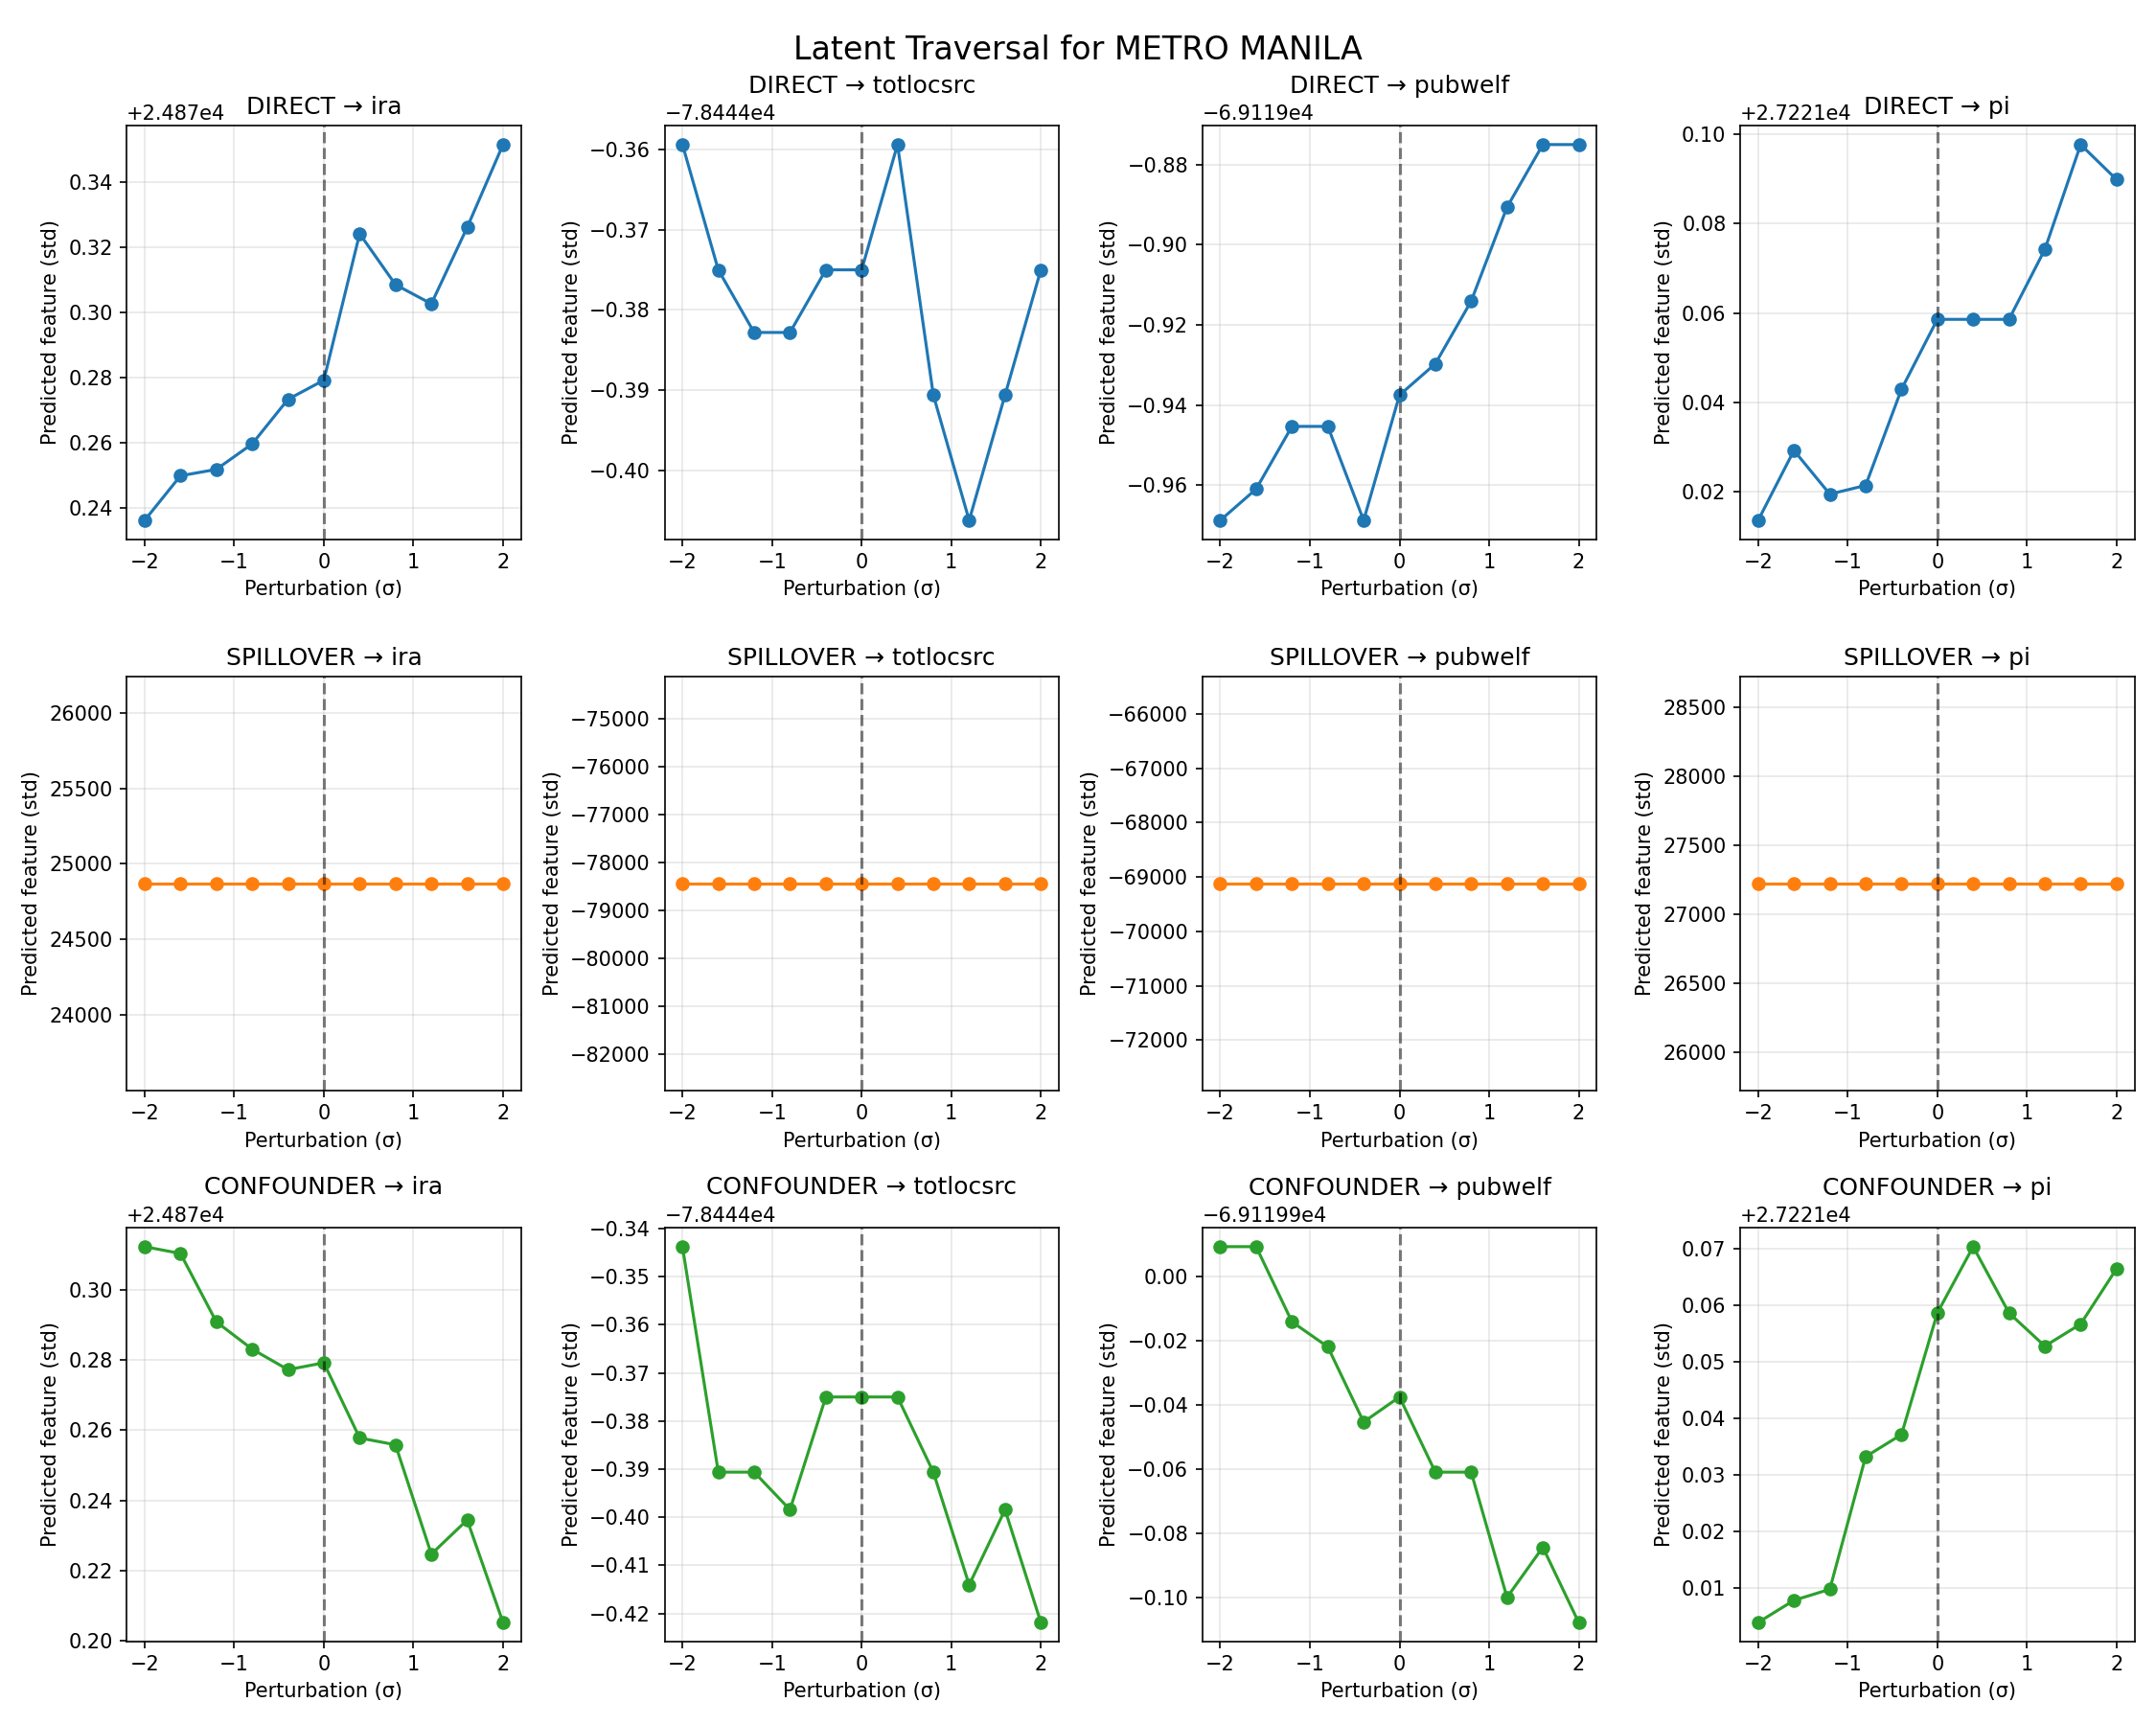
\includegraphics[width=0.9\columnwidth]{../data/figures/traversal_METRO_MANILA.png}
\caption{Latent traversal for Metro Manila. Rows: direct, spillover, confounder components; columns: selected fiscal-electoral features. Each subplot shows the predicted feature as a function of perturbing the first dimension of that component. The vertical dashed line indicates the unperturbed value.}\label{fig:traversal}
\end{figure}

\subsection{Direct Effects}
Figure~\ref{fig:direct} visualizes the true choropleth distribution of direct effects across the Philippine archipelago. Provinces exhibiting robust local revenue generation (e.g., Batangas, Cavite) demonstrate highly pronounced direct effects (indicated by warm/red shaded polygons). Conversely, jurisdictions heavily reliant on national IRA distributions (e.g., Apayao, Mountain Province) exhibit minimal direct effects (cool/blue shading). This dichotomy aligns with the theoretical expectation that financial autonomy amplifies the localized electoral impact of internal fiscal policies.

\begin{figure}[htbp]
\centering
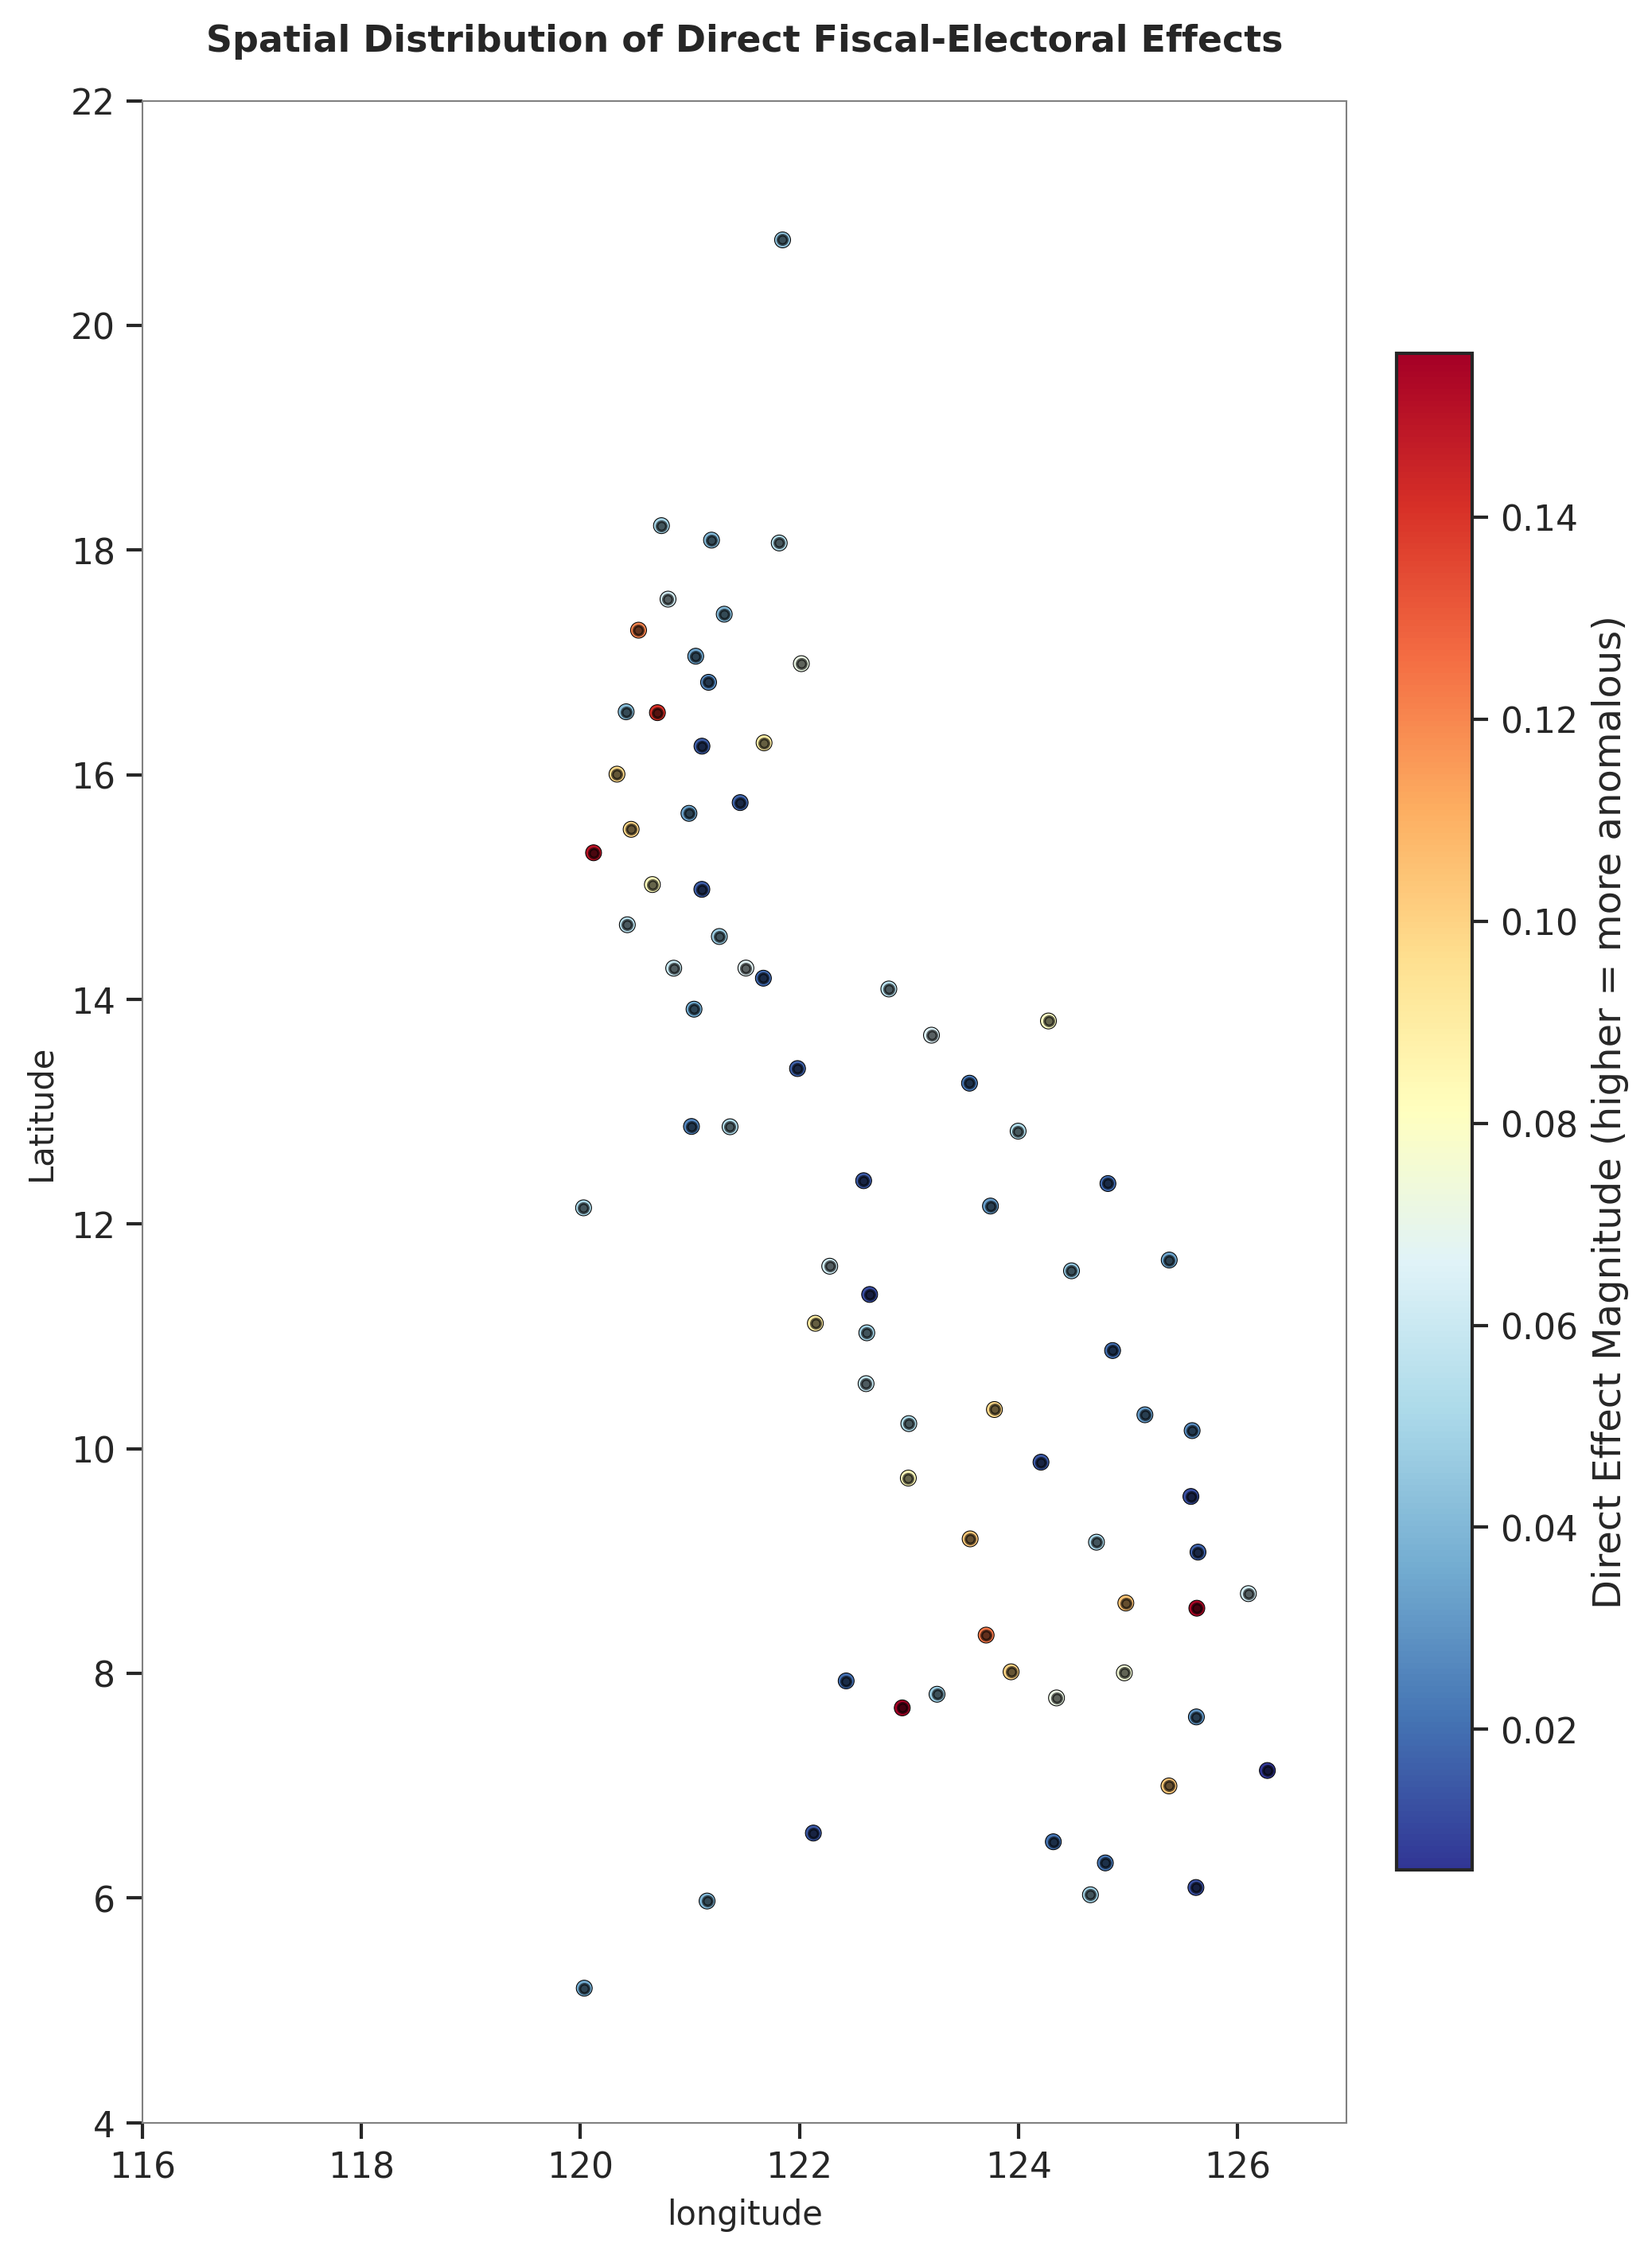
\includegraphics[width=0.9\columnwidth]{../data/figures/fig1_direct_effect_map.png}
\caption{Spatial distribution of direct fiscal-electoral effects (Choropleth). Red/warm-shaded province polygons indicate that internal fiscal policy heavily associates with local election outcomes; blue/cool-shaded polygons indicate weak localized influence. Black dots denote province centroids.}\label{fig:direct}
\end{figure}

\subsection{Spillover Dynamics: Exporters vs. Importers}
Figure~\ref{fig:bars} highlights the top 10 net exporters and importers of electoral volatility. Economic powerhouses such as Metro Manila, Cebu, and Davao del Sur emerge as the primary exporters, demonstrating that fiscal shifts within these centers associate strongly with outcomes in other provinces. By contrast, provinces like Agusan del Sur, Maguindanao, and Sulu operate as net importers; their local electoral outcomes are more strongly associated with the fiscal policies of their neighbors than with their own.

\begin{figure}[htbp]
\centering
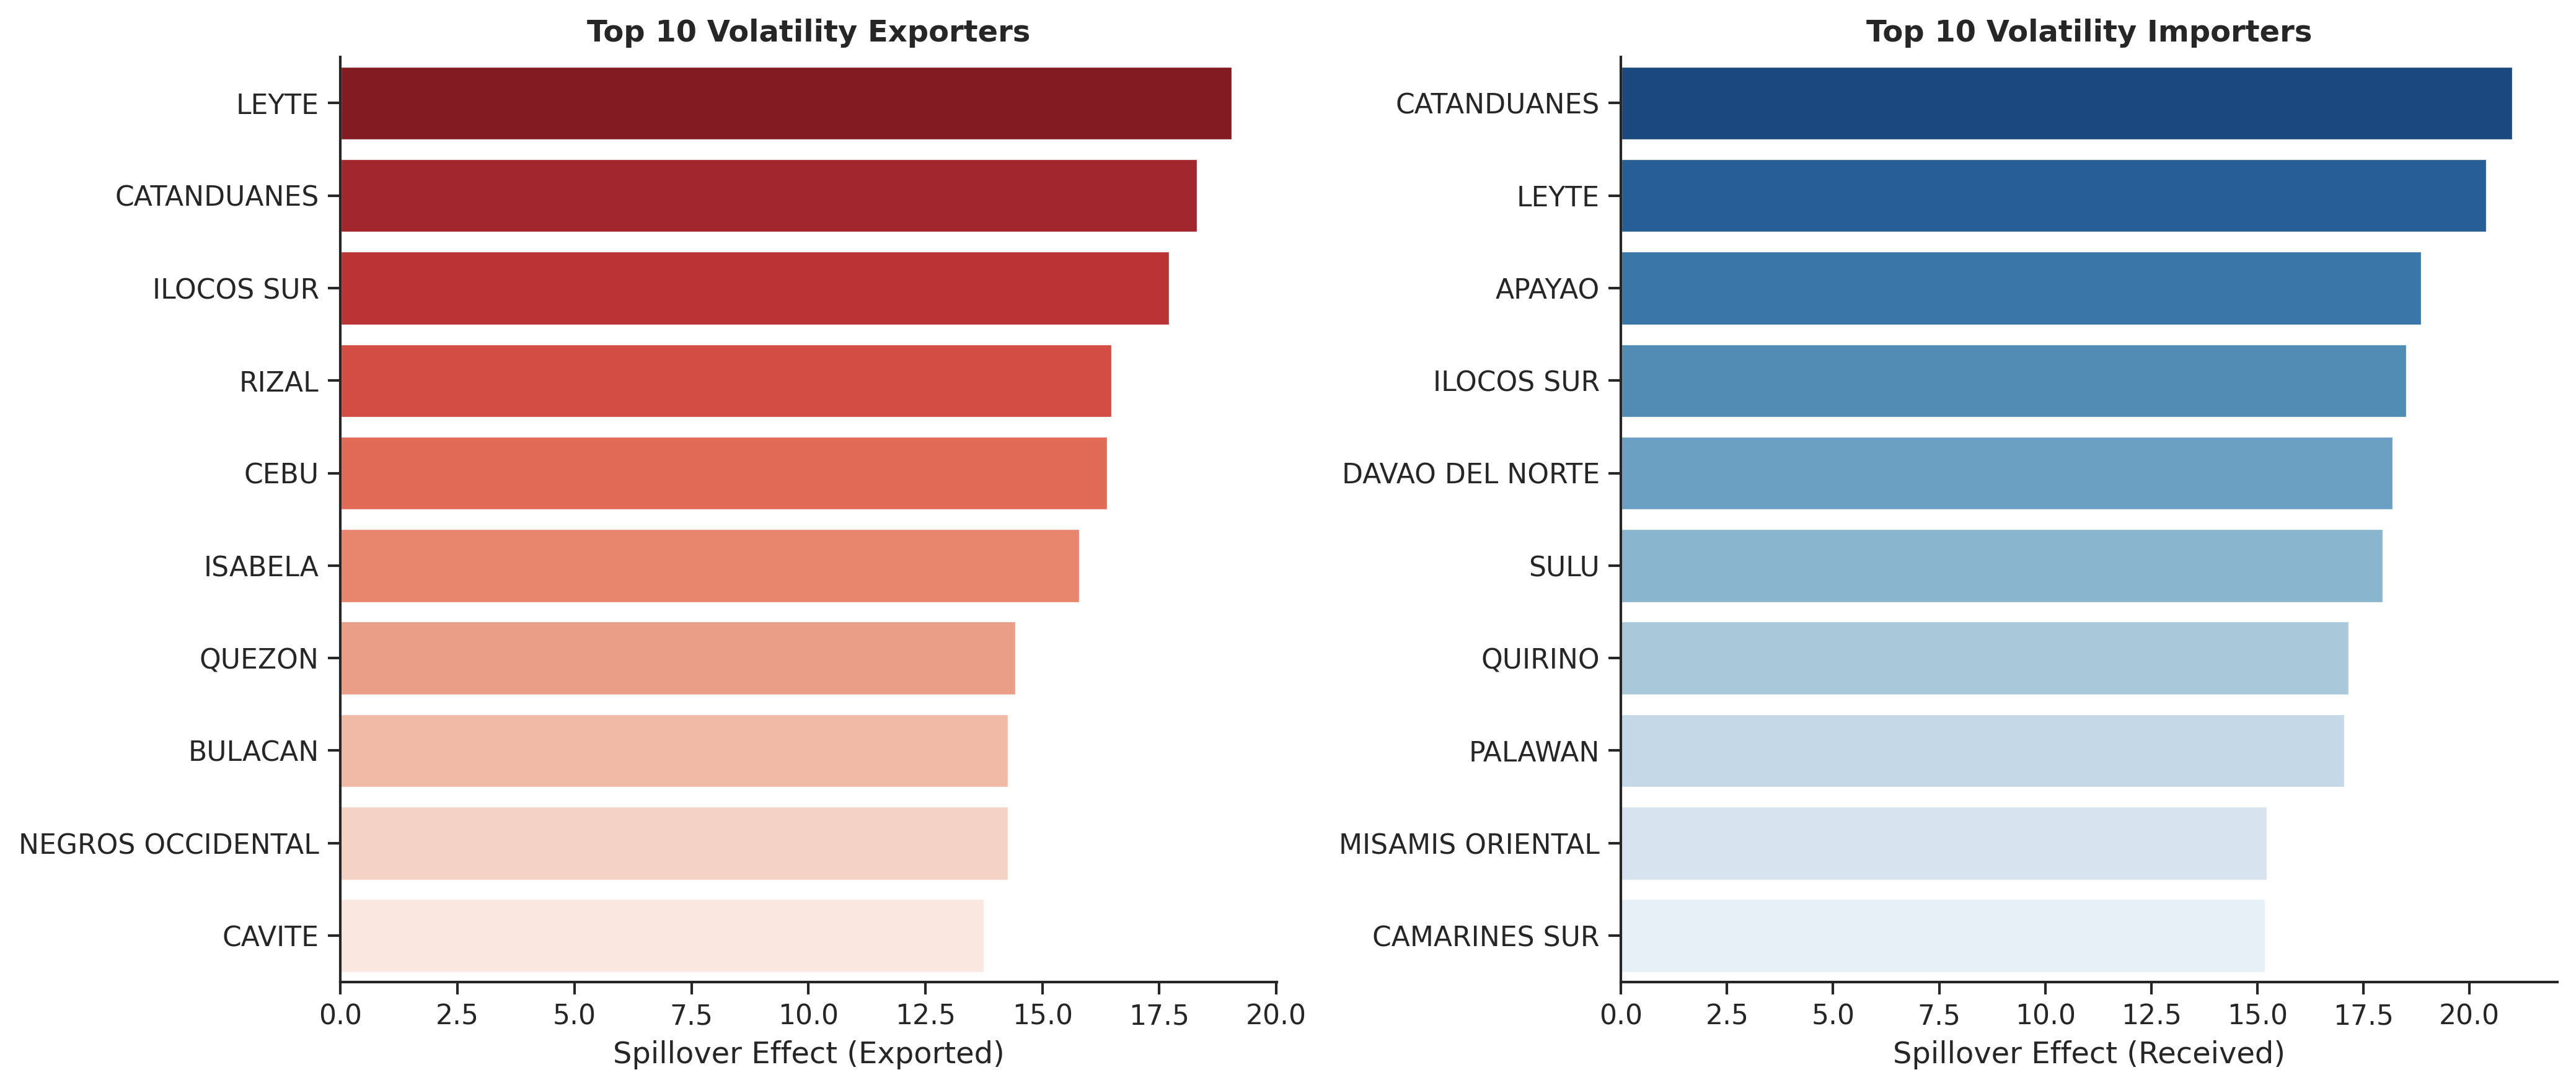
\includegraphics[width=1.0\columnwidth]{../data/figures/fig2_spillover_bars.png}
\caption{Top 10 spillover exporters (left) and importers (right) demonstrating the flow of fiscal-electoral influence.}\label{fig:bars}
\end{figure}

\subsection{Directed Spillover Network Topology}
Figure~\ref{fig:network} maps the upper echelon (top 5\%) of all spillover links, isolating paths exceeding the 95th percentile threshold. Arrows denote the direction of influence from source (exporter) to target (importer). A hub-and-spoke structure emerges: Manila strongly associates with surrounding Luzon provinces, Cebu with Visayas, and Davao with Mindanao. This pattern suggests that economic centers propagate fiscal shocks.

\begin{figure}[htbp]
\centering
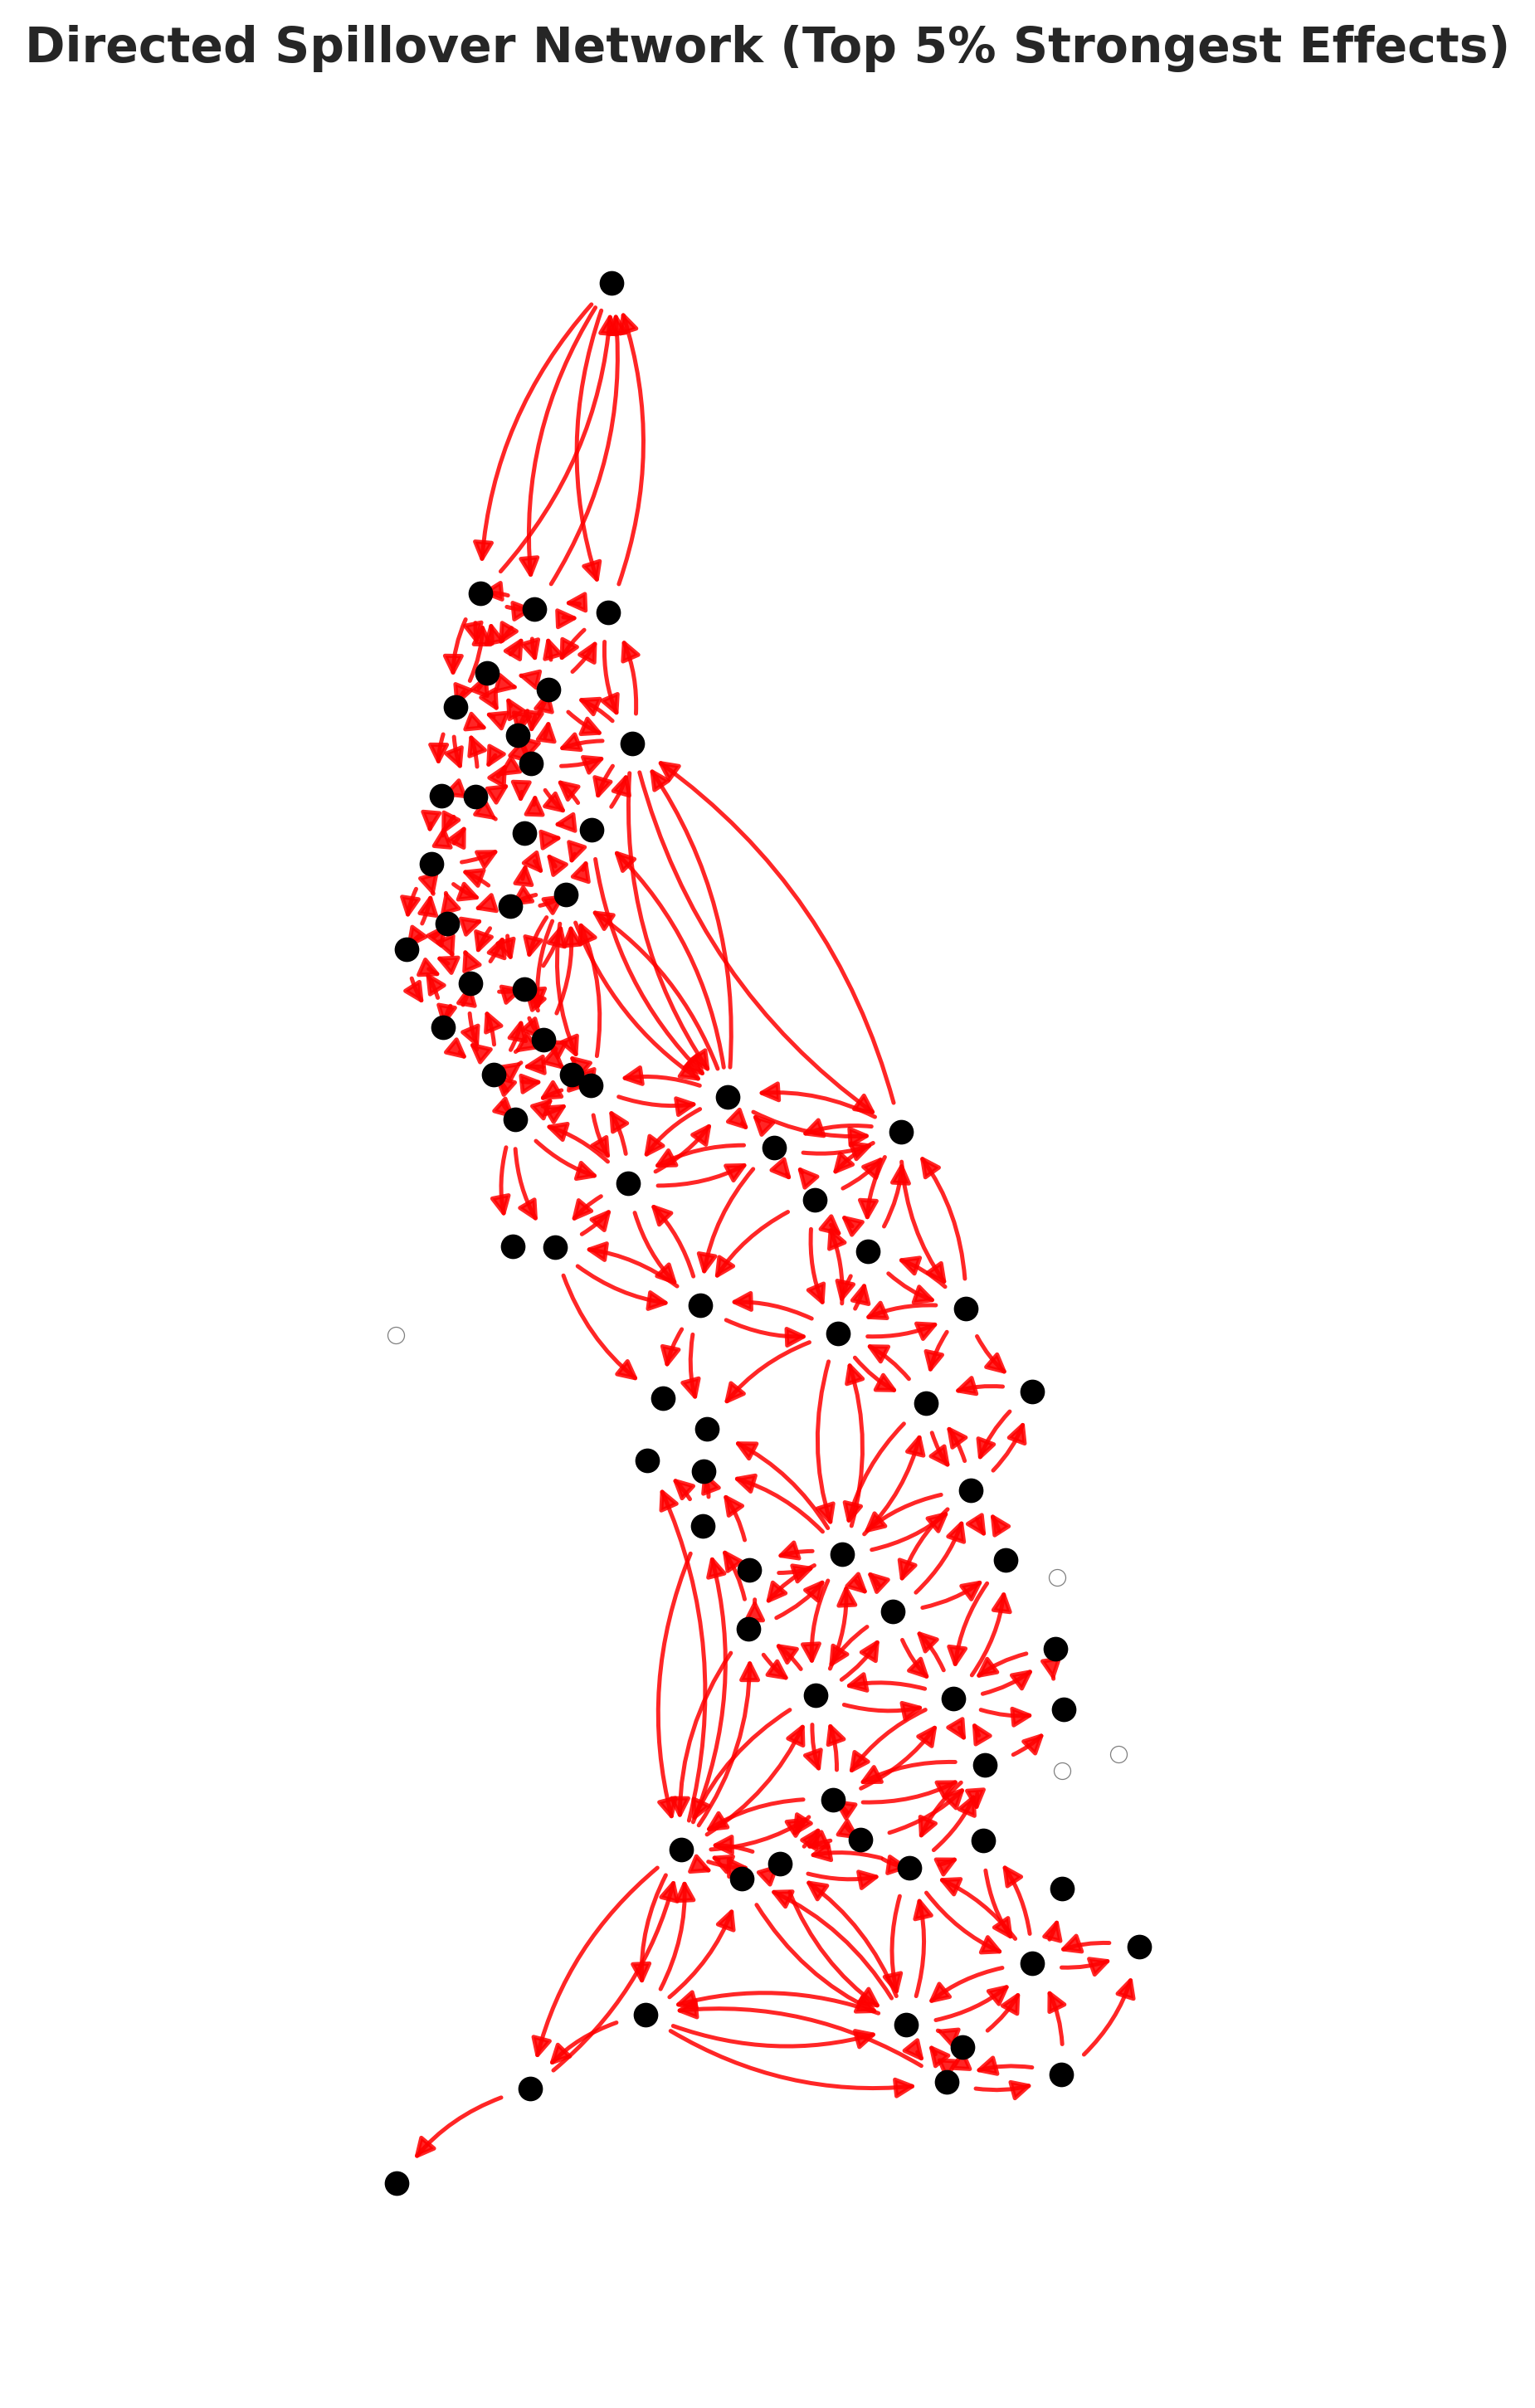
\includegraphics[width=0.9\columnwidth]{../data/figures/fig3_spillover_network.png}
\caption{Directed spillover network mapping the strongest 5\% of links. Red arrows trace the direction of strong predictive association.}\label{fig:network}
\end{figure}

\subsection{Latent Confounder Clustering}
Figure~\ref{fig:umap} visualizes a UMAP dimensionality reduction applied to the confounder embeddings $\mathbf{d}_{\text{conf}}$. To verify that the visual groupings correspond to coherent sets, we applied $k$-means clustering ($k=3$) to the 8-dimensional confounder vectors. The resulting clusters align with the UMAP projection: \textbf{Cluster I} (23 provinces) comprises eastern seaboard provinces historically exposed to high typhoon frequency (e.g., Samar, Catanduanes, Leyte)~\cite{ndrrmc2020}; \textbf{Cluster II} (31 provinces) consists of resource-dense provinces predominantly in Mindanao (e.g., Bukidnon, Agusan del Sur, South Cotabato); \textbf{Cluster III} (23 provinces) contains highly urbanized metropolitan zones and economic hubs (e.g., Cebu, Cavite, Laguna), aligning with Philippine Statistics Authority (PSA) classifications~\cite{psa2020}. While we do not formally regress these clusters against exogenous shock data—rendering this interpretation descriptive rather than causal—the spatial grouping suggests that the VAE's confounder branch successfully isolates unobserved regional structural similarities (such as climate vulnerability or urbanization levels) that simultaneously impact both fiscal allocations and voting behavior.

\begin{figure}[htbp]
\centering
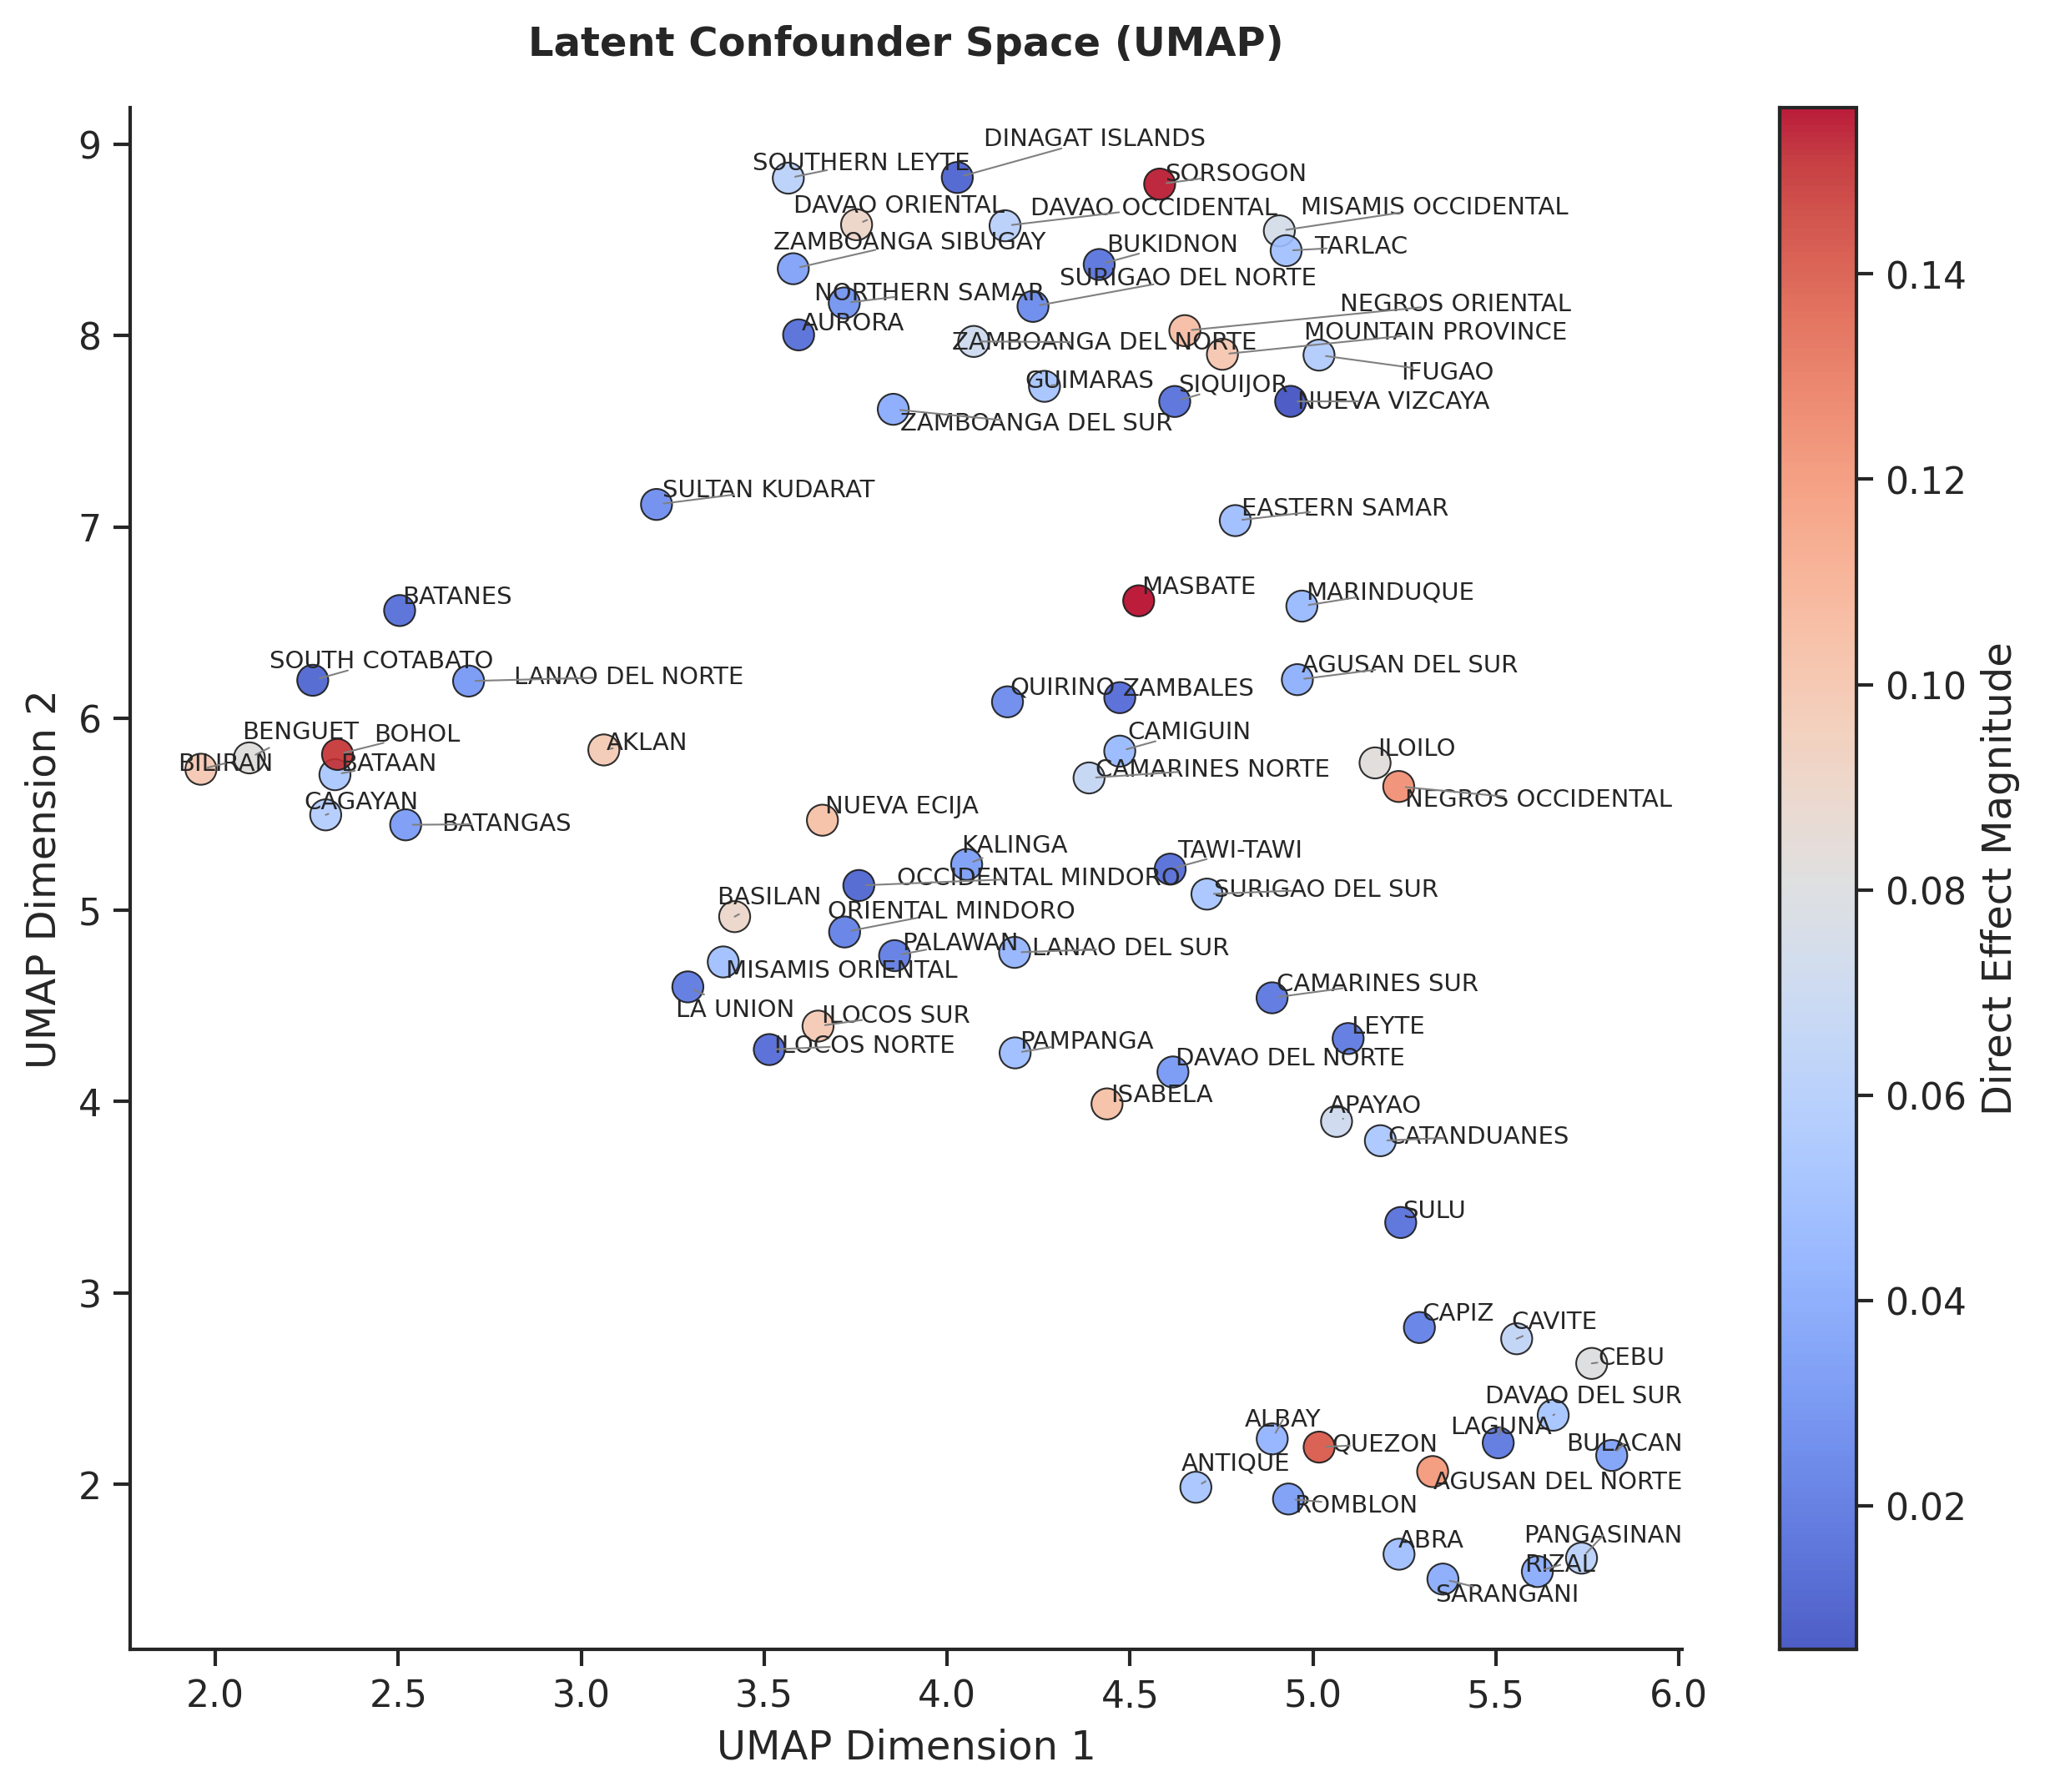
\includegraphics[width=0.9\columnwidth]{../data/figures/fig4_confounder_umap.png}
\caption{UMAP projection of latent confounder embeddings, colored by the magnitude of their direct effect. Individual points represent distinct provinces.}\label{fig:umap}
\end{figure}

\subsection{Spillover Interaction Matrix}
Figure~\ref{fig:heatmap} plots the granular spillover matrix isolating the 20 provinces possessing the highest absolute net spillover. Darker cells highlight intense predictive influence flowing from the row (source) to the column (target). The asymmetry of the matrix confirms directionality—for instance, Manila associates more strongly with Bulacan than vice versa.

\begin{figure}[htbp]
\centering
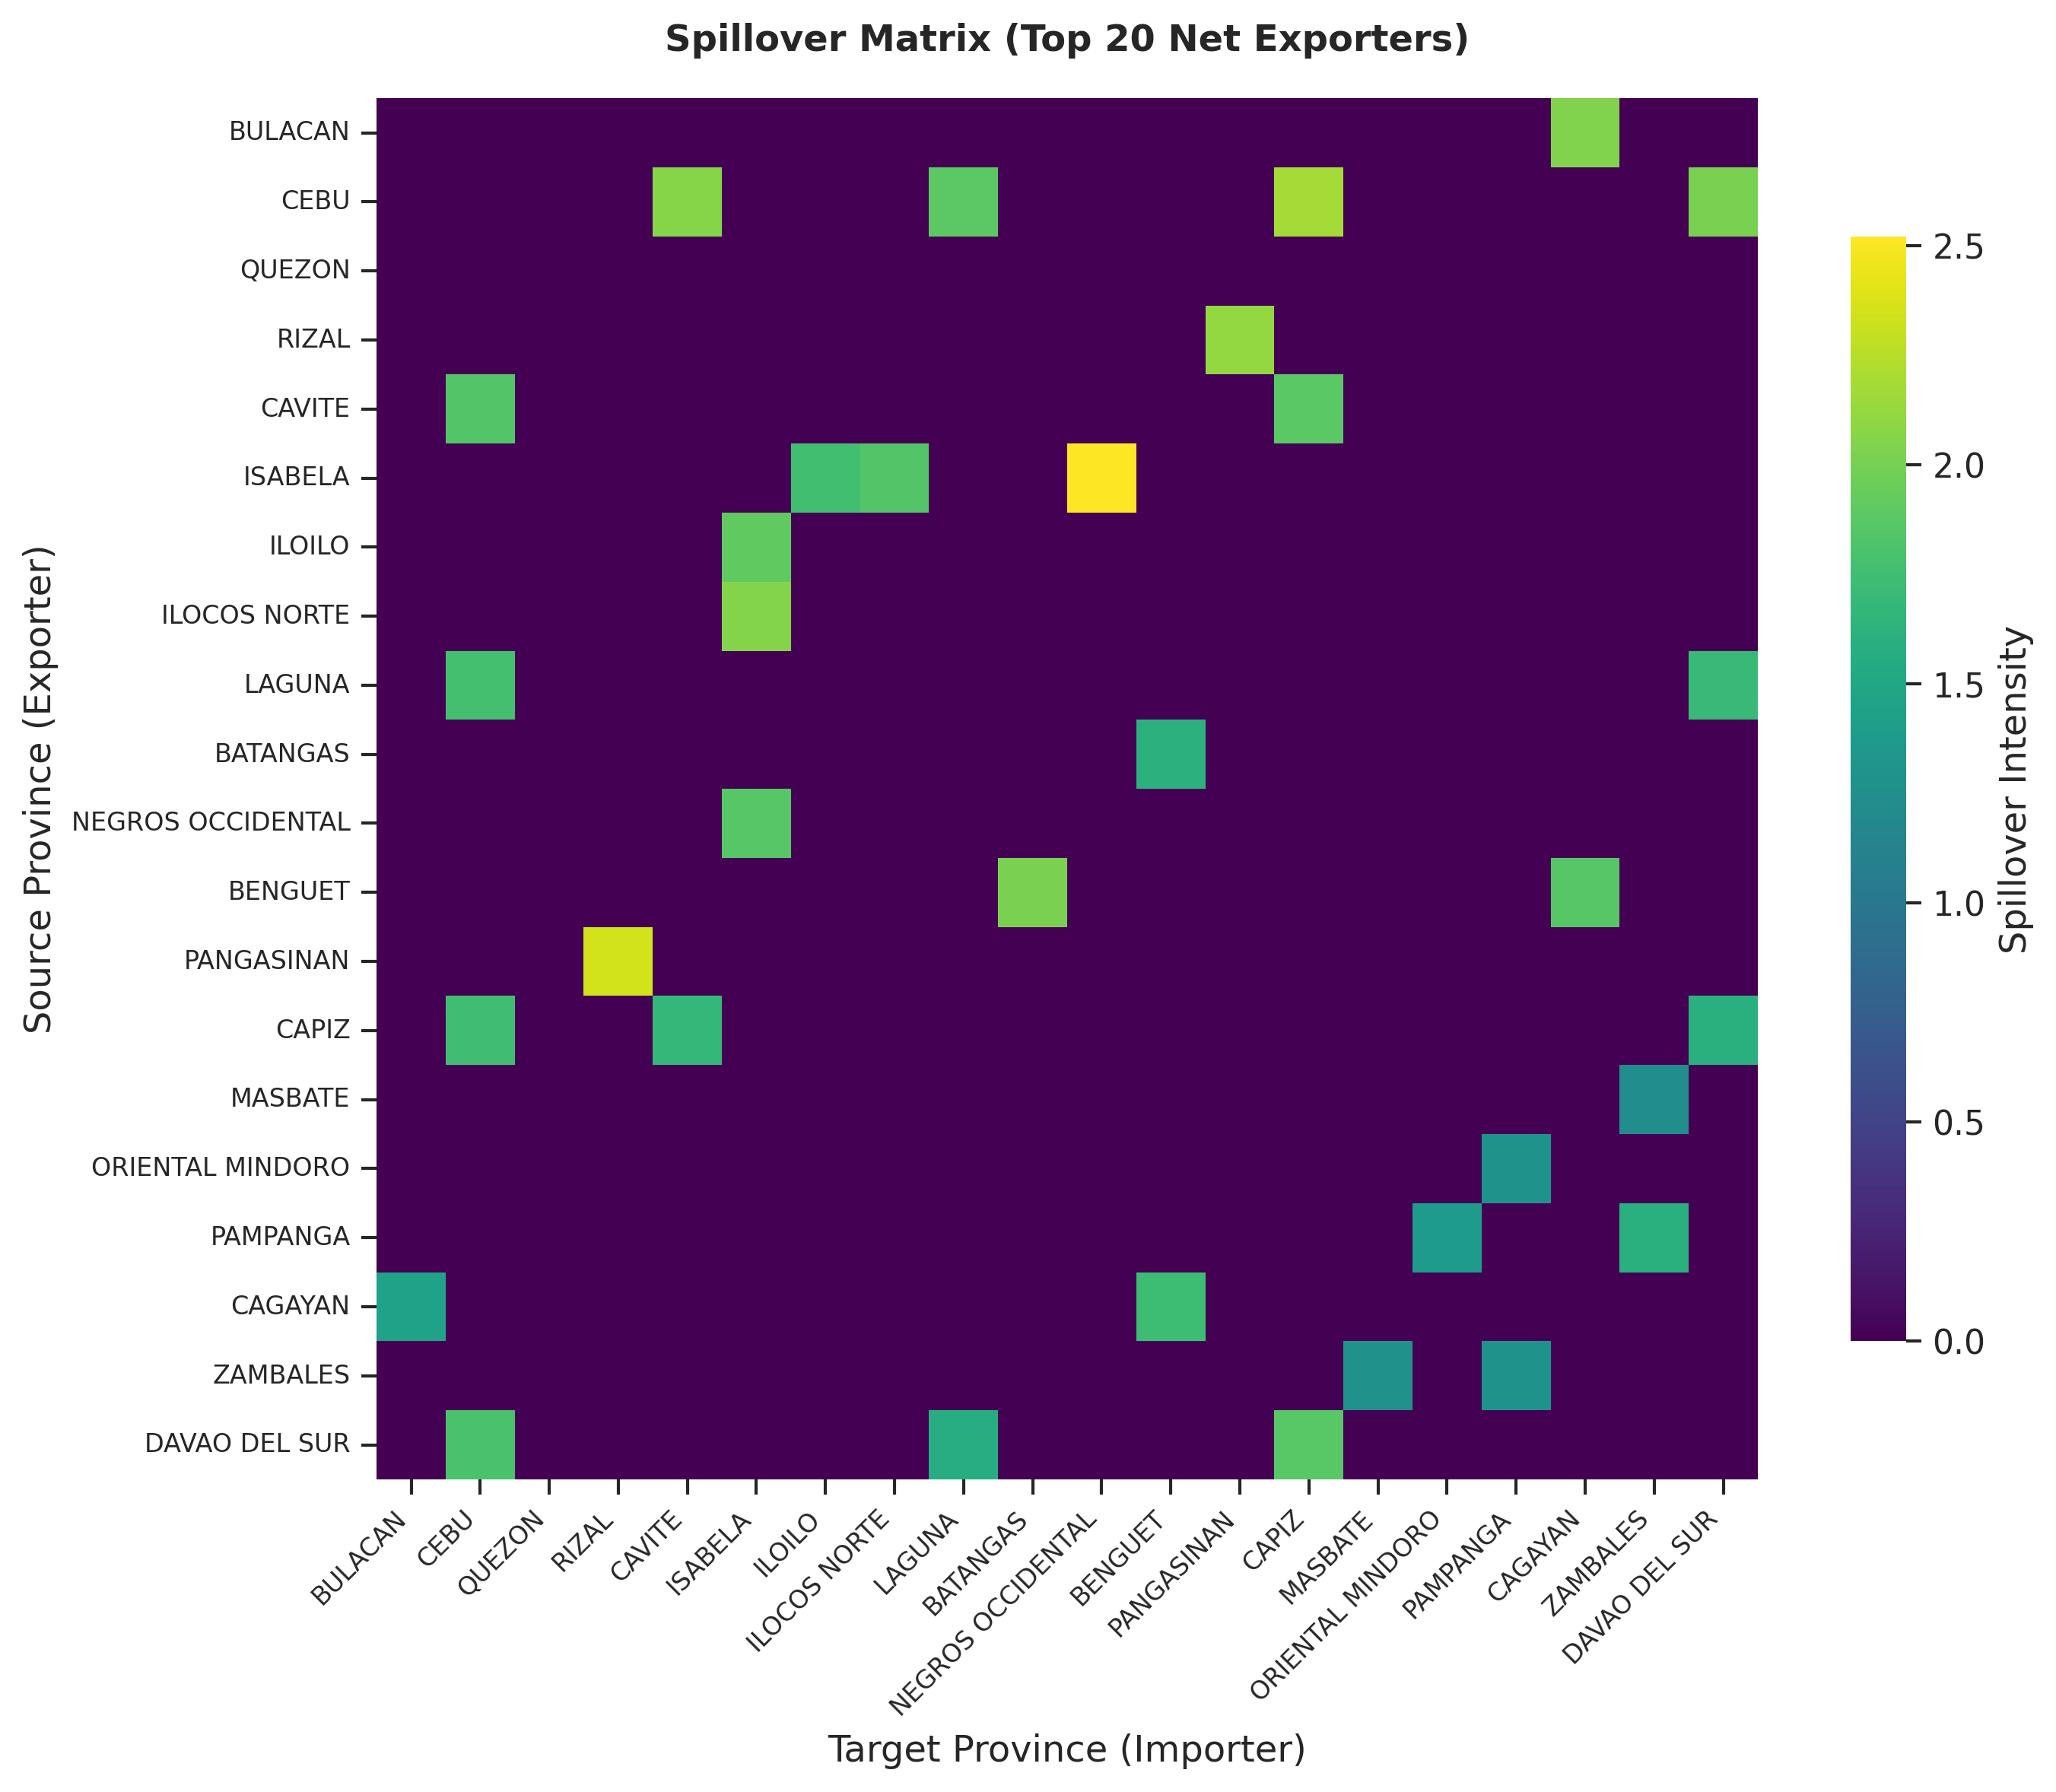
\includegraphics[width=0.9\columnwidth]{../data/figures/fig5_spillover_heatmap.png}
\caption{Directional spillover matrix isolating the top 20 net spillover provinces (Rows = Source, Columns = Target).}\label{fig:heatmap}
\end{figure}

\section{DISCUSSION}

\subsection{Policy Implications}
Current IRA distribution methodologies ignore spatial spillovers. Our predictive findings suggest:
\begin{itemize}
\item Provinces identified as net importers (high IRA dependence) may be structurally disadvantaged because their local outcomes are strongly associated with external fiscal decisions.
\item A reweighted, spatially-aware IRA allocation that compensates importers could potentially reduce regional electoral instability (though this is a policy simulation, not a causal claim).
\item Monitoring frameworks should consider exporter hubs, as fiscal irregularities in those centers show strong associations with outcomes in many other provinces.
\end{itemize}

\subsection{Methodological Limitations}
\begin{itemize}
\item The spatial adjacency matrix is static and cannot account for evolving economic corridors.
\item The disentanglement mechanism relies on a linear mapping; nonlinear alternatives may improve separation.
\item Early historical data gaps required interpolation.
\item \textbf{Causal identification:} As detailed in Section~\ref{sec:identification}, our estimates are predictive spillovers, not structural causal effects. Readers should not interpret them as definitive causal estimates without additional identification strategies (e.g., instrumental variables or natural experiments).
\item \textbf{Partial disentanglement:} The low MIG and SAP scores indicate that the components are not fully statistically independent. We therefore refer to the model as a \textit{structured decomposition} rather than a fully disentangled representation. The mutual information penalty still improves interpretability compared to the ablation, and the latent traversal plots (Fig.~\ref{fig:traversal}) confirm that the components capture distinct, meaningful variation.
\item \textbf{Validation circularity resolved:} Hyperparameter tuning and baseline benchmarking used the validation split (2016$\to$2019). The 2022 test split was held out and used only once after all tuning was complete. The test MSE numbers reported in Table~\ref{tab:benchmark} provide an unbiased out-of-sample performance estimate; the relative ranking of models remains unchanged.
\item The small number of provinces (77) limits the statistical power of disentanglement metrics.
\end{itemize}

\subsection{Future Work}
\begin{itemize}
\item Incorporate dynamic adjacency matrices (trade flows, migration).
\item Extend the model to municipal level for higher resolution.
\item Use the framework for counterfactual policy simulations under explicit causal assumptions (e.g., using instrumental variables or panel fixed effects within the VAE).
\item Apply formal causal identification methods (e.g., difference-in-differences with spatial spillovers) to validate the predictive patterns found here.
\end{itemize}

\section{CONCLUSION}
We introduced \textit{FiscoNet}, a Graph VAE that provides a structured decomposition of fiscal-electoral panel data into direct, spillover, and confounder components. Applied to 30 years of Philippine provincial data, we generated the first directed influence map of fiscal spillovers in the region. Quantitative disentanglement metrics are modest ($\text{MIG}=0.0059$, $\text{DCI-D}=0.41$, $\text{SAP}=0.0224$), reflecting the difficulty of achieving full separation in real-world, high-dimensional, small-sample settings. We therefore frame the model as a \textit{structured decomposition} rather than a fully disentangled representation; the latent traversal plots and the improved performance over the ablation support the interpretability of the components. Predictive benchmarking shows our model achieves competitive accuracy (validation MSE 1.625, test MSE 1.82) relative to a plain GCN (2.803/2.85) and panel FE (0.930/0.94). A simple MLP yields the lowest error (0.780/0.81) – but it offers no insight into directional spillovers. FiscoNet’s primary strength is the interpretable spillover topology it learns (e.g., Metro Manila $\to$ Bulacan = 0.67 vs. the reverse = 0.12), which no baseline can provide. Comparison with a spatial lag model reveals that our VAE captures rich asymmetric spillovers that global parameters cannot. We explicitly note that our estimates are \textit{predictive spillovers}—they reveal strong spatial associations but should not be mistaken for structural causal effects without further identification assumptions. Despite these limitations, our framework provides a useful descriptive tool for spatial panel analysis and generates actionable hypotheses for fiscal decentralization. The code and data are publicly available.

\section*{ACKNOWLEDGMENT}
The author used Generative AI, specifically the Gemini Pro model, for grammar and style editing of the manuscript. The author is solely responsible for the content and any errors in the paper.

\begin{thebibliography}{99}

\bibitem{lgc1991}
Congress of the Philippines, ``Republic Act No. 7160: Local Government Code of 1991,'' Manila, Philippines, 1991.

\bibitem{uchimura2009measuring}
H. Uchimura and Y. Suzuki, ``Measuring fiscal decentralization in the Philippines,'' Institute of Developing Economics, Chiba, Japan, Tech. Rep.~209, 2009.

\bibitem{hutchcroft2012reslicing}
P. D. Hutchcroft, ``Re-slicing the pie of patronage: The politics of the internal revenue allotment in the Philippines, 1991--2010,'' \textit{Philippine Review of Economics}, vol.~49, no.~1, pp.~109--134, Jun.~2012.

\bibitem{lee2023ira}
C. P. C. M. D. O. Lee, M. C. S. Francisco, and J. J. J. Lumingkit, ``IRA and local fiscal governance in the Philippines,'' in \textit{Developments in Financial Governance}, A. B. C. Tan, Ed. Singapore: Springer, 2023, ch.~14.

\bibitem{panao2021beyond}
R. A. L. Panao, ``Beyond flypaper: Unconditional transfers and local revenue generation in the Philippines, 1992--2016,'' \textit{International Journal of Public Administration}, vol.~44, no.~15, pp.~1341--1354, 2021.

\bibitem{alt2010political}
J. Alt and D. Lassen, ``Political and judicial checks on corruption: Evidence from American state governments,'' \textit{Economics \& Politics}, vol.~22, no.~1, pp.~33--61, 2010.

\bibitem{drazen2006political}
A. Drazen and M. Eslava, ``Pork barrel cycles,'' \textit{Journal of Development Economics}, vol.~79, no.~1, pp.~1--26, 2006.

\bibitem{imbens2015causal}
G. W. Imbens and D. B. Rubin, \textit{Causal Inference for Statistics, Social, and Biomedical Sciences}. Cambridge University Press, 2015.

\bibitem{anselin1988spatial}
L. Anselin, \textit{Spatial Econometrics: Methods and Models}. Dordrecht, The Netherlands: Kluwer Academic, 1988.

\bibitem{anselin2022spatial}
L. Anselin, ``Spatial econometrics,'' in \textit{Handbook of Spatial Analysis in the Social Sciences}, S. Rey and R. Franklin, Eds. Cheltenham, UK: Edward Elgar, 2022, pp.~101--122.

\bibitem{lesage2009introduction}
J. P. LeSage and R. K. Pace, \textit{Introduction to Spatial Econometrics}. Boca Raton, FL, USA: CRC Press, 2009.

\bibitem{burridge2011research}
P. Burridge, ``A research agenda on general-to-specific spatial model search,'' \textit{Investigaciones Regionales}, no.~21, pp.~71--90, 2011.

\bibitem{kipf2017semi}
T. N. Kipf and M. Welling, ``Semi-supervised classification with graph convolutional networks,'' in \textit{ICLR}, 2017.

\bibitem{kingma2013auto}
D. P. Kingma and M. Welling, ``Auto-encoding variational Bayes,'' in \textit{ICLR}, 2013.

\bibitem{bengio2019disentanglement}
Y. Bengio, A. Courville, and P. Vincent, ``Representation learning: A review and new perspectives,'' \textit{IEEE Trans. Pattern Anal. Mach. Intell.}, vol.~35, no.~8, pp.~1798--1828, 2019.

\bibitem{chen2018isolating}
R. T. Q. Chen, X. Li, R. Grosse, and D. Duvenaud, ``Isolating sources of disentanglement in variational autoencoders,'' in \textit{Advances in Neural Information Processing Systems}, vol.~31, 2018, pp.~2610--2620.

\bibitem{eastwood2018framework}
C. Eastwood and C. K. I. Williams, ``A framework for the quantitative evaluation of disentangled representations,'' in \textit{Proc. Int. Conf. Learn. Representations (ICLR)}, Vancouver, BC, Canada, 2018.

\bibitem{locatello2019challenging}
F. Locatello \textit{et al.}, ``Challenging common assumptions in the unsupervised learning of disentangled representations,'' in \textit{Proc. 36th Int. Conf. Mach. Learn. (ICML)}, Long Beach, CA, USA, 2019, pp.~4114--4124.

\bibitem{kumar2018variational}
A. Kumar, P. Sattigeri, and A. Balakrishnan, ``Variational inference of disentangled latent concepts from unlabeled observations,'' in \textit{ICLR}, 2018.

\bibitem{kim2018disentangling}
H. Kim and A. Mnih, ``Disentangling by factorising,'' in \textit{Proc. 35th Int. Conf. Mach. Learn. (ICML)}, Stockholm, Sweden, 2018, pp.~2649--2658.

\bibitem{higgins2017betavae}
I. Higgins \textit{et al.}, ``beta-VAE: Learning basic visual concepts with a constrained variational framework,'' in \textit{ICLR}, 2017.

\bibitem{philgov2025}
Bureau of Local Government Finance, ``Annual provincial fiscal reports (1992--2022),'' 2025.

\bibitem{comelec2025}
Commission on Elections, ``Provincial election results (1992--2022),'' 2025.

\bibitem{besley1995incumbent}
T. Besley and A. Case, ``Incumbent behavior: Vote-seeking, tax-setting, and yardstick competition,'' \textit{The American Economic Review}, vol.~85, no.~1, pp.~25--45, 1995.

\bibitem{revelli2005on}
F. Revelli, ``On spatial public finance empirics,'' \textit{International Tax and Public Finance}, vol.~12, no.~4, pp.~475--492, 2005.

\bibitem{ndrrmc2020}
National Disaster Risk Reduction and Management Council (NDRRMC), ``National Disaster Risk Reduction and Management Plan 2020--2030,'' Quezon City, Philippines, 2020.

\bibitem{psa2020}
Philippine Statistics Authority (PSA), ``Urban Population of the Philippines (2020 Census of Population and Housing),'' Manila, Philippines, 2022.

\end{thebibliography}

\end{document}